\chapter{Testowanie i ocena aplikacji} W niniejszym rozdziale przedstawiono proces testowania aplikacji oraz ocenę poprawności jej działania pod względem funkcjonalnym i niefunkcjonalnym. Omówione zostały podejścia wykorzystane w testach jednostkowych, integracyjnych, testy wydajnościowe oraz testy end-to-end. Celem testowania było upewnienie się, że wszystkie warstwy systemu współpracują prawidłowo, a aplikacja spełnia postawione wymagania w warunkach zbliżonych do rzeczywistych obciążeń. \section{Wprowadzenie do testowania aplikacji} Testowanie stanowi kluczowy element procesu tworzenia oprogramowania, umożliwiający wykrycie błędów oraz weryfikację poprawności zaimplementowanych funkcjonalności na wczesnym etapie. W ramach tego projektu zastosowano różne poziomy testów, aby uzyskać pewność co do jakości kodu: \begin{itemize}
\item \textbf{Testy jednostkowe} –Testy jednostkowe sprawdzają pojedyncze jednostki kodu. Pozwalają sprawdzić logikę wybranego fragmentu kodu w oderwaniu od kontekstu aplikacji (np. metodę serwisu aktualizującą statystyki lub walidującą dane wejściowe) \cite{effective-unit-testing}.
\item \textbf{Testy integracyjne} – sprawdzają, czy współpraca wielu komponentów (warstwa web, logika, dostęp do danych, mechanizmy bezpieczeństwa) przebiega poprawnie w uruchomionym kontekście aplikacji. \cite{spring-docs}
\item \textbf{Testy wydajnościowe} – oceniają zachowanie aplikacji przy wzrastającym obciążeniu i równoległych użytkownikach, aby upewnić się, że czasy odpowiedzi mieszczą się w akceptowalnych granicach \cite{jmeter-docs}.
\end{itemize} Tak wielopoziomowe podejście do testowania umożliwia wykrycie różnych klas błędów od drobnych pomyłek w logice pojedynczej metody, przez problemy z konfiguracją kontekstu Spring, aż po ewentualne wąskie gardła w wydajności. \section{Testy jednostkowe} Testy jednostkowe zostały napisane z użyciem frameworka JUnit 5, który jest obecnie standardem w ekosystemie Java. Do izolowania zależności wykorzystano bibliotekę Mockito, pozwalającą na tworzenie próbnych obiektów (moków) zastępujących np. warstwę repozytorium podczas testowania serwisu, lub warstwę serwisu podczas testowania kontrolera \cite{mockito-docs}. Dzięki temu można skupić się na logice danej jednostki kodu, nie przejmując się działaniem pozostałych komponentów (które są zasymulowane). Przykładowo, testy jednostkowe objęły klasy:
\begin{itemize}
\item \textbf{Serwisy} – np. \texttt{StatsService}, gdzie sprawdzono czy metoda aktualizująca statystyki poprawnie odczytuje dane z repozytoriów i zapisuje zaktualizowane statystyki. Zastosowano tutaj \textit{stub} na metodach repozytoriów \cite{mockito-docs, junit-docs}(\texttt{postRepository}, \texttt{userRepository}, itp.) zwracające z góry ustalone wartości, by zasymulować określony stan systemu, a następnie weryfikowano, czy serwis wywołuje metodę zapisu statystyk dokładnie raz z poprawnymi parametrami.
\item \textbf{Kontrolery} – testowane zarówno metodami bezpośredniego wywołania, jak i z użyciem Spring MockMVC. W pierwszym podejściu tworzono instancję kontrolera i za pomocą moków podstawiano zależności (np. \texttt{UserRepository}, \texttt{PasswordEncoder}), a następnie wywoływano metodę kontrolera tak, jakby obsługiwała żądanie. Sprawdzano zwracany widok oraz efekty uboczne (np. czy nowy użytkownik został zapisany w repozytorium po rejestracji). W drugim podejściu (MockMVC) uruchamiano wbudowany serwer Tomcat w trybie testowym i wykonywano sztuczne zapytania HTTP do endpointów, sprawdzając kod odpowiedzi i fragmenty wygenerowanej strony. \cite{spring-docs}
\item \textbf{Repozytoria} – ponieważ repozytoria Hazelcast nie korzystają z klasycznego mechanizmu ORM ani bazy SQL, testy jednostkowe repozytoriów polegały głównie na sprawdzeniu logiki metod filtrujących. Np. \texttt{ClassSignUpRepository.findBySchoolClassIdAndUserId} filtruje kolekcję zapisów, więc utworzono kilka obiektów \texttt{ClassSignUp} w kontrolowanej mapie i upewniono się, że metoda znajduje właściwy obiekt lub zwraca \texttt{Optional.empty()} gdy brak dopasowania \cite{hazelcast-docs}.
\end{itemize}
Poniżej przedstawiono fragment przykładowego testu jednostkowego dla serwisu statystyk \texttt{StatsService}, demonstrującego użycie Mockito do symulacji repozytoriów i weryfikacji zachowania:
\begin{lstlisting}[language=Java,
  caption={test kodu aktualizowania statystyk. Źródło: opracowanie własne},
  label={lst:testStatisticUpdater},
  captionpos=b]
@Test
void shouldUpdateStatisticsCorrectly() {
// Symulacja wartości zwracanych przez repozytoria:
when(postRepository.count()).thenReturn(10L);
when(userRepository.countByRole("TEACHER")).thenReturn(2L);
when(userRepository.countByRole("USER")).thenReturn(5L);
when(commentRepository.count()).thenReturn(20L);
// Wywołanie testowanej metody:
statsService.updateStatistics();
// Weryfikacja, że statystyki zostały zapisane (4 statystyki do zapisania):
verify(statsRepository, times(4)).save(any(AppStatistic.class));
}
\end{lstlisting} W powyższym teście założono, że w systemie jest 10 postów, 2 nauczycieli, 5 zwykłych użytkowników i 20 komentarzy. Po wywołaniu \texttt{updateStatistics()} oczekujemy, że serwis spróbuje zapisać każdą z czterech statystyk (postCount, teacherCount, userCount, commentCount) dokładnie raz – stąd \texttt{verify} z \texttt{times(4)} na \texttt{statsRepository.save(...)}. Wykorzystanie mechanizmów Mockito pozwoliło na izolację testowanej metody od faktycznej bazy danych i innych serwisów  test jest szybki i deterministyczny. \section{Testy integracyjne} Testy integracyjne przeprowadzono z wykorzystaniem wbudowanych możliwości Spring Boot Test. Uruchamiając kontekst całej aplikacji w trybie testowym, można symulować rzeczywiste scenariusze użytkownika, sprawdzając czy wszystkie warstwy (od kontrolera, przez serwisy, po repozytoria i magazyn danych) działają wspólnie poprawnie. W projekcie wykorzystano głównie podejście \textbf{end-to-end}, gdzie testy integracyjne zachowywały się jak klienci aplikacji korzystający z niej przez protokół HTTP. Do realizacji takich testów zastosowano:
\begin{itemize}
  \item \texttt{SpringBootTest} z \texttt{webEnvironment=RANDOM\_PORT} --
dzięki \texttt{RANDOM\_PORT} testy uruchamiają aplikację na wolnym porcie, co pozwala na rzeczywisty dostęp HTTP do endpointów.
  \item \texttt{TestRestTemplate} --  klient HTTP z pakietu Spring Boot Test, umożliwiający wykonywanie żądań HTTP do uruchomionej aplikacji.
  \item profil \texttt{test} -- w testach aktywowano profil testowy, który
    używa osobnej konfiguracji Hazelcast (mniejsza liczba danych
    inicjalnych, wyłączone zadania cykliczne poprzez
    \texttt{spring.task.scheduling.enabled=false}, aby testy były
    deterministyczne).
\end{itemize}
 Przykładem testu integracyjnego może być sprawdzenie działania strony głównej aplikacji: \begin{lstlisting}[language=Java,
  caption={integracyjny test. Źródło: opracowanie własne},
  label={lst:integrationTest},
  captionpos=b]
@SpringBootTest(webEnvironment = SpringBootTest.WebEnvironment.RANDOM_PORT)
@ActiveProfiles("test")
class ApplicationIntegrationTests {
@Autowired
private TestRestTemplate restTemplate;
@Test
void homePageShouldLoadSuccessfully() {
ResponseEntity<String> response = restTemplate.getForEntity("/", String.class);
assertEquals(HttpStatus.OK, response.getStatusCode());
assertTrue(response.getBody().contains("Welcome to MyEduShare"));
}
}
\end{lstlisting} 
W powyższym teście uruchamiamy aplikację, wykonujemy zapytanie GET na
\texttt{"/"} (strona główna) i sprawdzamy, czy odpowiedź ma kod 200OK oraz
czy zwrócona treść HTML zawiera oczekiwany fragment (np. tytuł lub
charakterystyczny tekst powitalny strony). Taki test potwierdza, że
podstawowa ścieżka (wejście na stronę główną) działa prawidłowo-- aplikacja
się uruchamia, kontroler główny zwraca widok, a mechanizmy szablonów
poprawnie generują stronę.

Bardziej złożone testy integracyjne zostały stworzone dla typowych
scenariuszy użycia, opisanych w poprzednim rozdziale. Na przykład
przygotowano test end-to-end symulujący cały przepływ:
\textit{nauczyciel tworzy nowy kurs i zadanie $\to$ student rejestruje się i
zapisuje na ten kurs $\to$ student przesyła rozwiązanie zadania $\to$
nauczyciel pobiera i ocenia rozwiązanie $\to$ sprawdzenie, że ocena jest
zapisana}. Tego typu test (zaimplementowany w klasie
\texttt{TeacherStudentFlowE2eTest}) wykorzystuje \texttt{TestRestTemplate}
do wykonywania kolejnych żądań POST/GET, naśladując akcje formularzy (np.
przesyłając dane rejestracji w żądaniu POST do
\texttt{/perform\_register}, logując różne konta poprzez
\texttt{TestRestTemplate} z odpowiednimi ciasteczkami sesyjnymi itp.) \cite{spring-docs}. Po
serii akcji test weryfikuje stan bazy-- np. sprawdza, czy w repozytorium
\texttt{TaskSubmissionRepository} pojawił się wpis z oceną nauczyciela. Takie
kompleksowe testy dają dużą pewność, że kluczowe funkcjonalności aplikacji
działają poprawnie w całym przekroju systemu.

W trakcie testów integracyjnych aplikacja korzystała z tej samej bazy
Hazelcast (tyle że w trybie „test”, z osobną konfiguracją) co w normalnym
działaniu. Oznacza to, że wszystkie
operacje na danych w testach były wykonywane również w pamięci (co
zapewniło szybkość testów i identyczne warunki działania jak w
środowisku produkcyjnym aplikacji). Podejście to upraszcza testy-- brak
translacji do innej technologii (SQL) oznacza, że testujemy dokładnie te
same ścieżki kodu co podczas realnego działania aplikacji \cite{hazelcast-docs}. Testy
integracyjne potwierdziły poprawne współdziałanie komponentów aplikacji:
wszystkie zaplanowane scenariusze (rejestracja, logowanie, dodawanie
postów, zapisy na kurs, przesyłanie zadań, oceny itp.) zakończyły się
wynikiem zgodnym z oczekiwaniami. Również obsługa błędnych ścieżek (np.
próba dostępu do zasobów bez autoryzacji, podwójna rejestracja z tym samym
e-mailem) została zweryfikowana-- aplikacja w takich przypadkach zwraca komunikaty lub kody błędów (kod 403) \cite{spring-docs}.

\section{Testy wydajnościowe}

Ostatnim etapem było zbadanie zachowania aplikacji pod obciążeniem. W tym celu przygotowano plan w Apache JMeter, który symuluje jednoczesne działania wielu użytkowników i pozwala mierzyć czasy odpowiedzi oraz stabilność przepływów \cite{jmeter-docs}. Skrypt odwzorowuje typowe ścieżki użytkowników aplikacji. Poniżej zwięzły opis kluczowych elementów planu testowego.

\begin{itemize}
  \item \textbf{HTTP Request Defaults} ---  konfiguracja hosta (np. \texttt{localhost:8080}),
        protokołu i bazowej ścieżki, ułatwia utrzymanie skryptu \cite{jmeter-docs}.
  \item \textbf{HTTP Cookie \& Cache Manager} --- podtrzymanie sesji zalogowanego użytkownika i obsługa ciasteczek oraz cache przeglądarki \cite{jmeter-docs}.
  \item \textbf{CSV Data Set Config} --- strzykiwanie danych wejściowych (loginy/hasła i identyfikatory zasobów): \texttt{users\_teachers.csv}, \texttt{post\_ids.csv}, \texttt{class\_ids.csv} itp. \cite{jmeter-docs}.
  \item \textbf{Pobranie i przekazanie CSRF} --- po wejściu na \texttt{/login} token CSRF jest wyekstrahowany z HTML i dołączany do żądań \texttt{POST} (nagłówek \texttt{X-CSRF-TOKEN} i/lub pole formularza), zgodnie z mechanizmem ochrony w Spring Security \cite{spring-docs}.
  \item \textbf{Korelacja identyfikatorów} — ID pobierane z plików CSV lub z odpowiedzi (HTML/JSON) i przekazywane do kolejnych kroków \cite{jmeter-docs}.
  \item \textbf{Korelacja identyfikatorów} ---  ID pobierane z plików CSV lub z odpowiedzi (HTML/JSON) i przekazywane do kolejnych kroków \cite{jmeter-docs}.
  \item \textbf{Przykładowe ścieżki API użyte podczas testów}:
    \begin{itemize}
      \item \emph{Logowanie:} \texttt{GET /login} $\rightarrow$ \texttt{POST /perform\_login}
            z tokenem CSRF i danymi z CSV.
      \item \emph{Dodanie posta (nauczyciel):} \texttt{POST /teacher/posts/new}
      \item \emph{Ocena posta (użytkownik):} \texttt{POST /posts/\{postId\}/rate}
    \end{itemize}
  \item \textbf{liczniki czasu} --- \emph{Uniform Random Timer} (np. 500--2000 ms) między akcjami,
        aby zasymulować naturalne tempo klikania \cite{jmeter-docs}.
  \item \textbf{Kontrola tempa} --- opcjonalny \emph{Constant Throughput Timer} oraz/lub
        \emph{Throughput Controller}, aby utrzymać docelową liczbę żądań \cite{jmeter-docs}.
  \item \textbf{Assercje} --- weryfikacja kodów odpowiedzi (200/302), obecności oczekiwanych elementów w plikach HTML/JSON,
        co potwierdza poprawność funkcjonalną ścieżek API.
  \item \textbf{Zapisy wyników} --- \emph{Simple Data Writer} do JTL (pełne dane pomiarowe) oraz raporty HTML \cite{jmeter-docs}.
\end{itemize}

Fragment struktury planu:

\begin{lstlisting}[caption={Fragment planu testów JMeter. Źródło: opracowanie własne},
  label={lst:jmeter-plan}, captionpos=b]
Test Plan
 +-- HTTP Request Defaults (http://localhost:8080)
 +-- HTTP Cookie Manager, HTTP Cache Manager
 +-- CSV Data Set: users_teachers.csv, post_ids.csv, class_ids.csv
 +-- Thread Group (VUs, ramp-up, duration)
 |   +-- GET /login  -> extract CSRF
 |   +-- POST /perform_login  (CSRF, credentials from CSV)
 |   +-- POST /teacher/posts/new  (CSRF, param title/content)
 |   +-- POST /teacher/classes/${CLASS_ID}/lessons/new  (CSRF)
 |   +-- POST /posts/${POST_ID}/comments  (CSRF, param text)
 |   +-- POST /posts/${POST_ID}/rate  (CSRF, param rating)
 |   +-- Simple Data Writer (results.jtl), HTML Report
\end{lstlisting}


\subsection{Parametry przykładowego testu wydajnościowego}

Poniżej zestawiono parametry biegu oraz krótkie uzasadnienie doboru wartości.

\begin{itemize}
  \item \textbf{Liczba równoczesnych użytkowników (VUs):}
        100, 250, 600, 1000 \;-- cztery poziomy obciążenia pozwalające ocenić trend skalowania.
  \item \textbf{Ramp-up:} 60~s (dla 100 VUs), 120~s (dla 250 VUs), 180~s (dla 600 VUs), 240~s (dla 1000 VUs);
        płynne narastanie wątków ogranicza skokowe zmiany i stabilizuje pomiary \cite{jmeter-docs}.
  \item \textbf{Czas trwania:} 10~min ciągłego wykonywania akcji (po ramp-up), co daje reprezentatywny przekrój próbek \cite{jmeter-docs}.
  \item \textbf{Tempo akcji (liczniki czasu):} losowe odstępy 0.5--2.0~s między krokami, aby zbliżyć się do realnego użycia aplikacji \cite{jmeter-docs}.
\item \textbf{Zakres endpointów:}
    \begin{itemize}
        \item \texttt{/perform\_login}
        \item \texttt{/teacher/posts/new}
        \item \texttt{/teacher/classes/\{classId\}/lessons/new}
        \item \texttt{/posts/\{postId\}/comments}
        \item \texttt{/posts/\{postId\}/rate}
    \end{itemize}
  \item \textbf{Dane wejściowe:} loginy i hasła z \texttt{users\_teachers.csv}, identyfikatory klas i postów
        (\texttt{class\_ids.csv}, \texttt{post\_ids.csv}); wartości pól (tytuł/treść/komentarz/ocena) parametryzowane.
  \item \textbf{CSRF i sesja:} token CSRF automatycznie pobierany z widoku logowania i dołączany do wszystkich żądań POST
        sesja jest utrzymywana przez \emph{HTTP Cookie Manager} \cite{jmeter-docs}.
  \item \textbf{Zapisy metryk:} pełne zapisy próbek w pliku JTL, raporty HTML z wartościami
        \emph{Mediana, Średnia, p90, Min, Max}.
\end{itemize}

W tak zdefiniowanym scenariuszu skrypt mierzy rzeczywiste czasowe koszty przetwarzania operacji.
\subsection{Wyniki szczegółowe: metryki dla kolejnych poziomów VUs}

Poniżej przedstawiono metryki czasów odpowiedzi (w~ms) dla czterech kluczowych operacji:
\textbf{Post} (dodanie posta), \textbf{Komentarz} (dodanie komentarza), \textbf{Logowanie} oraz  \textbf{Lekcja} (dodanie lekcji).
Dla każdego poziomu obciążenia (100/250/600/1000 VUs) pięć metryk: \emph{Mediana},
\emph{Średnia}, \emph{p90}, \emph{Min} oraz \emph{Max}.

\FloatBarrier
\clearpage

% ===================== 100 VUs =====================
\subsubsection{100 VUs} \begin{figure}[H]\centering 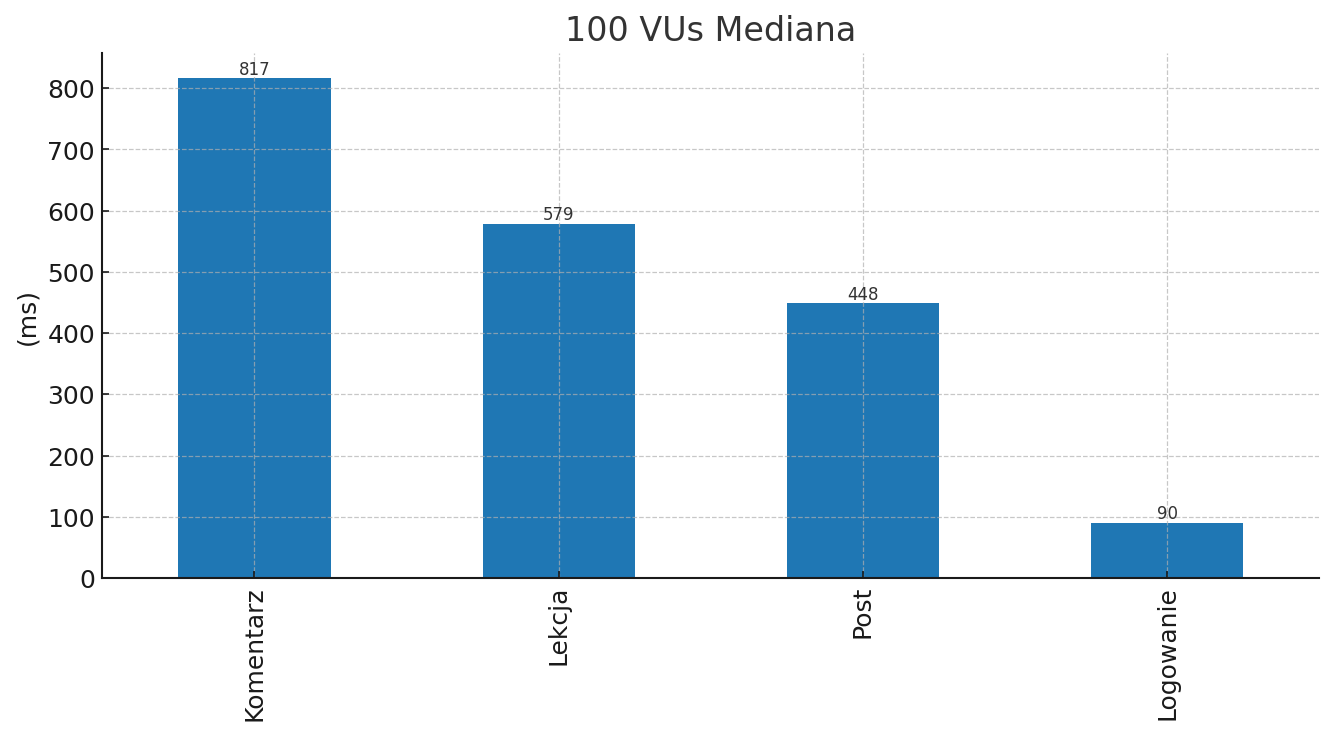
\includegraphics[width=\textwidth]{Dyplom-styl/chart_simple_100VU_mediana.png} \caption{100 VUs --- Mediana (ms). Źródło: Opracowanie własne}\label{fig:100-mediana} \end{figure} Mediany są niskie dla wszystkich operacji, operacje utrzymują komfortowy poziom opóźnień. \begin{figure}[H]\centering 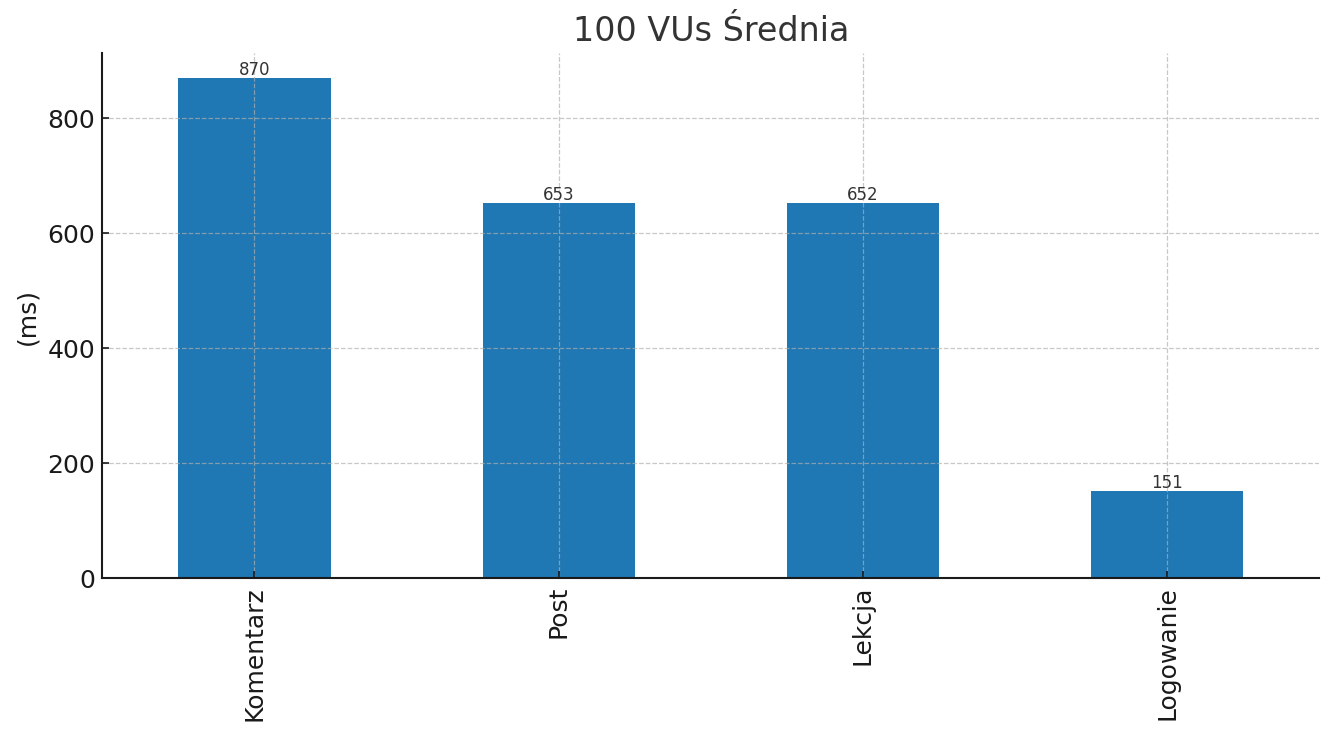
\includegraphics[width=\textwidth]{Dyplom-styl/chart_simple_100VU_srednia.png} \caption{100 VUs --- Średnia (ms). Źródło: Opracowanie własne}\label{fig:100-srednia} \end{figure} Średnie są zbliżone do median, co potwierdza stabilny profil obciążeń bez odchyleń. \begin{figure}[H]\centering 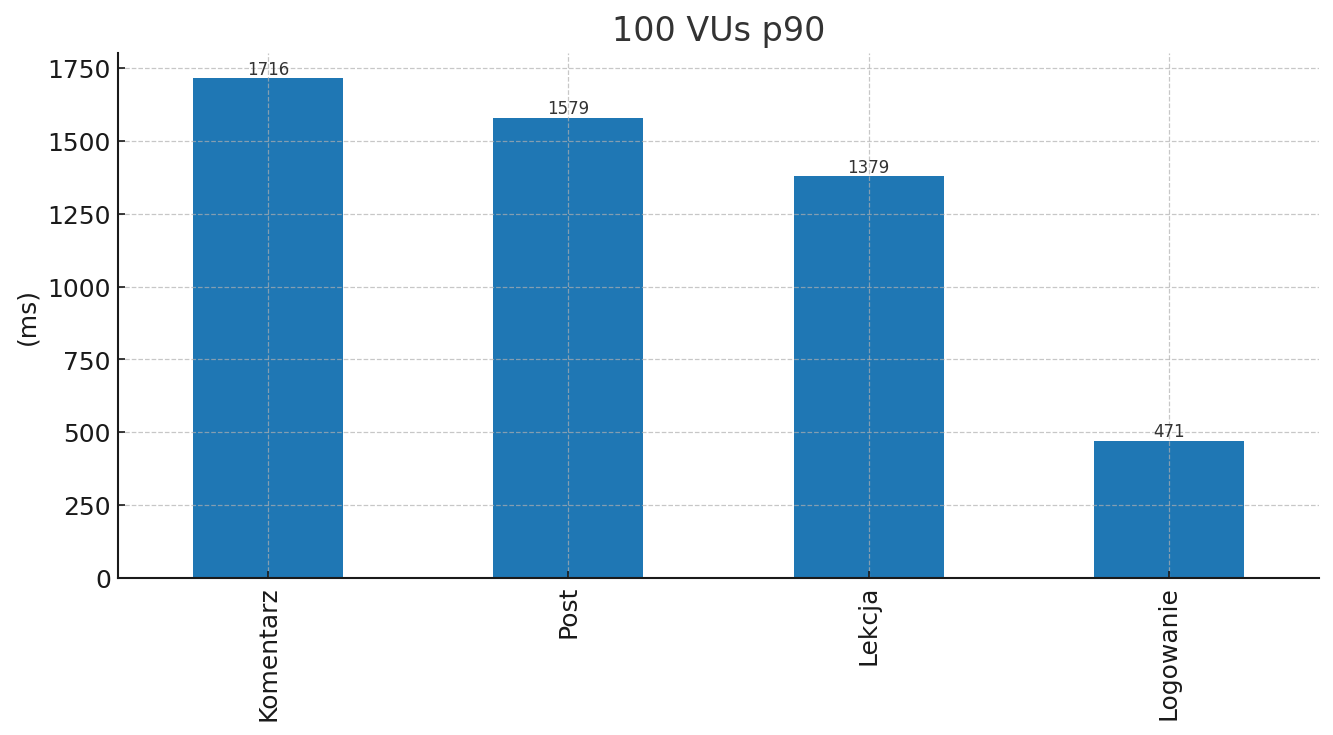
\includegraphics[width=\textwidth]{Dyplom-styl/chart_simple_100VU_p90.png} \caption{100 VUs --- p90 (ms). Źródło: Opracowanie własne}\label{fig:100-p90} \end{figure} p90 utrzymuje bezpieczny dystans od median, rezerwa wydajności jest wyraźna. \begin{figure}[H]\centering 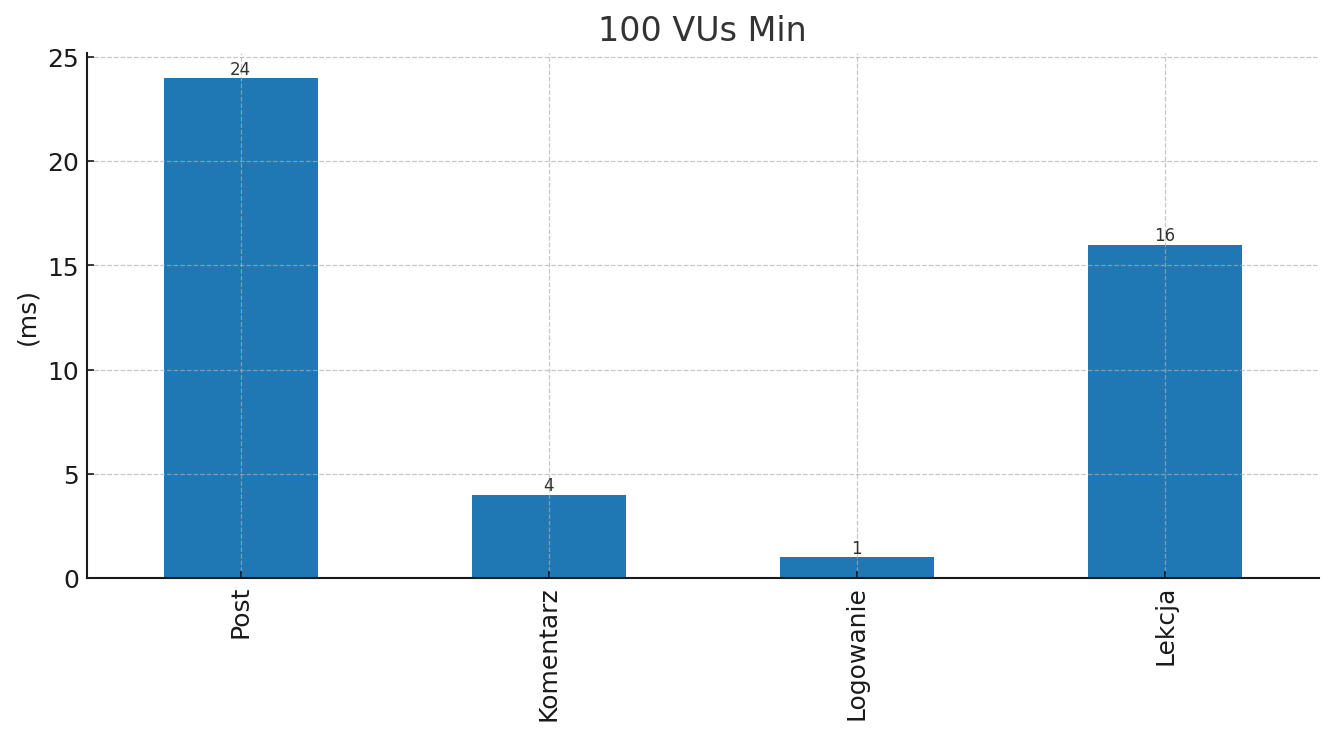
\includegraphics[width=\textwidth]{Dyplom-styl/chart_100VU_min_clean.png} \caption{100 VUs --- Min (ms). Źródło: Opracowanie własne }\label{fig:100-min} \end{figure} Minimalne czasy potwierdzają niskie koszty, żądań i szybką obsługę w pamięci.
\begin{figure}[H]\centering 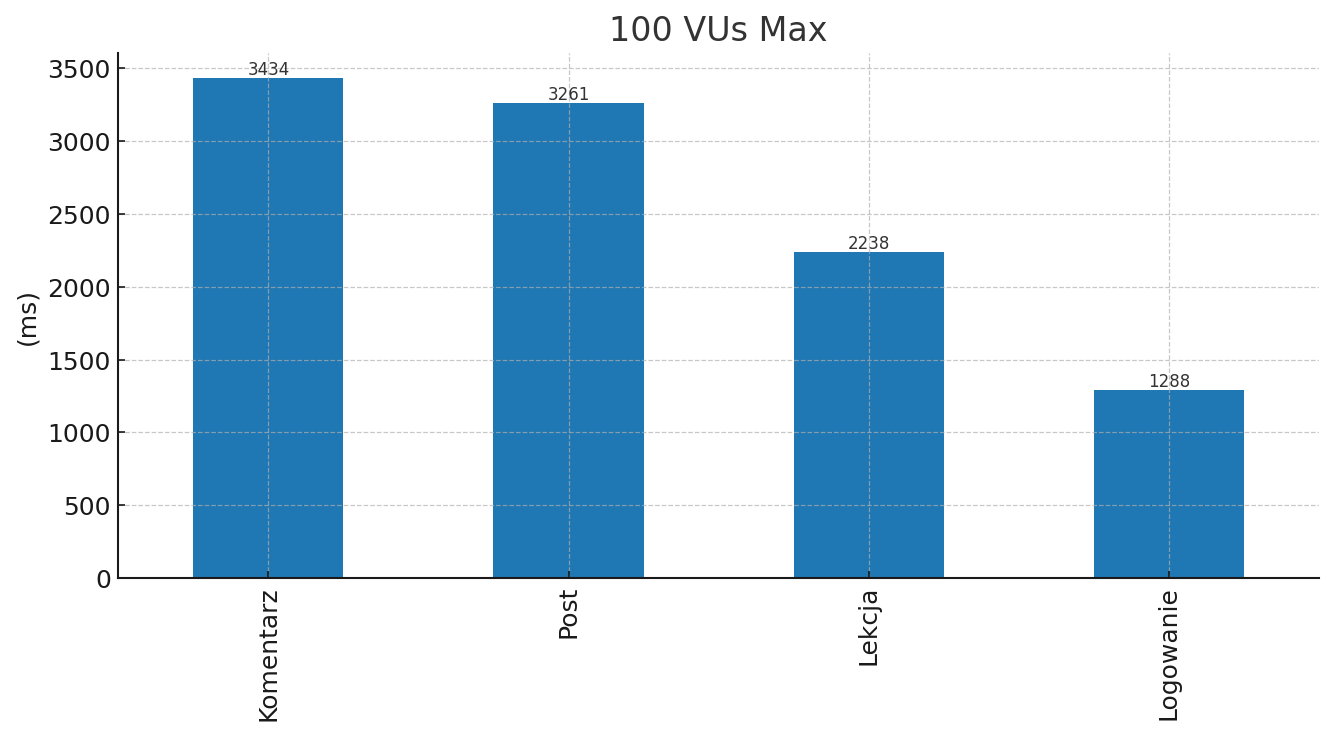
\includegraphics[width=\textwidth]{Dyplom-styl/chart_simple_100VU_max.png} \caption{100 VUs --- Max (ms). Źródło: Opracowanie własne }\label{fig:100-min} \end{figure} Maksymalne wartości występują okazjonalnie nie wpływając na odczucie podczas używania aplikacji.
% ===================== 250 VUs =====================
\subsubsection{250 VUs}

\begin{figure}[H]\centering
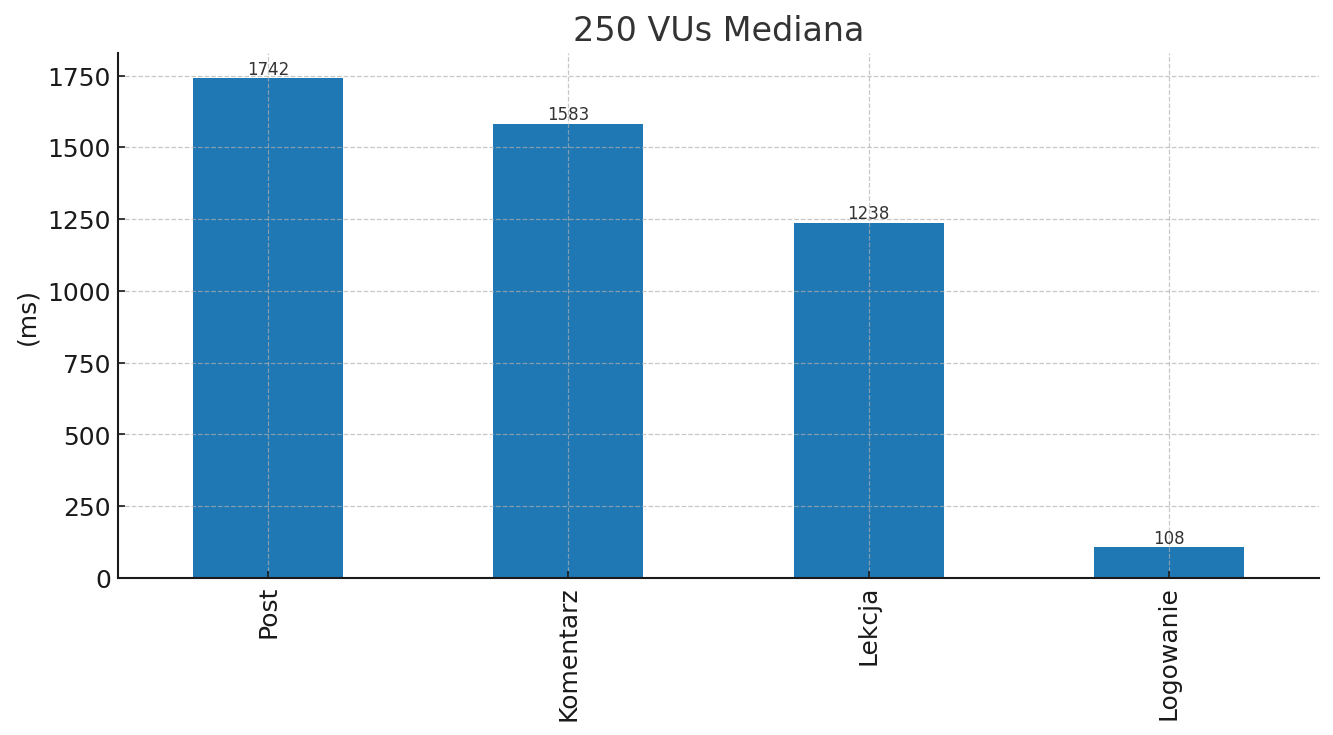
\includegraphics[width=\textwidth]{Dyplom-styl/chart_250VU_mediana.png}
\caption{250 VUs --- Mediana (ms). Źródło: Opracowanie własne}\label{fig:250-mediana}
\end{figure}
Wzrost obciążenia skutkuje przewidywalnym, łagodnym wzrostem median, brak skoków.

\begin{figure}[H]\centering
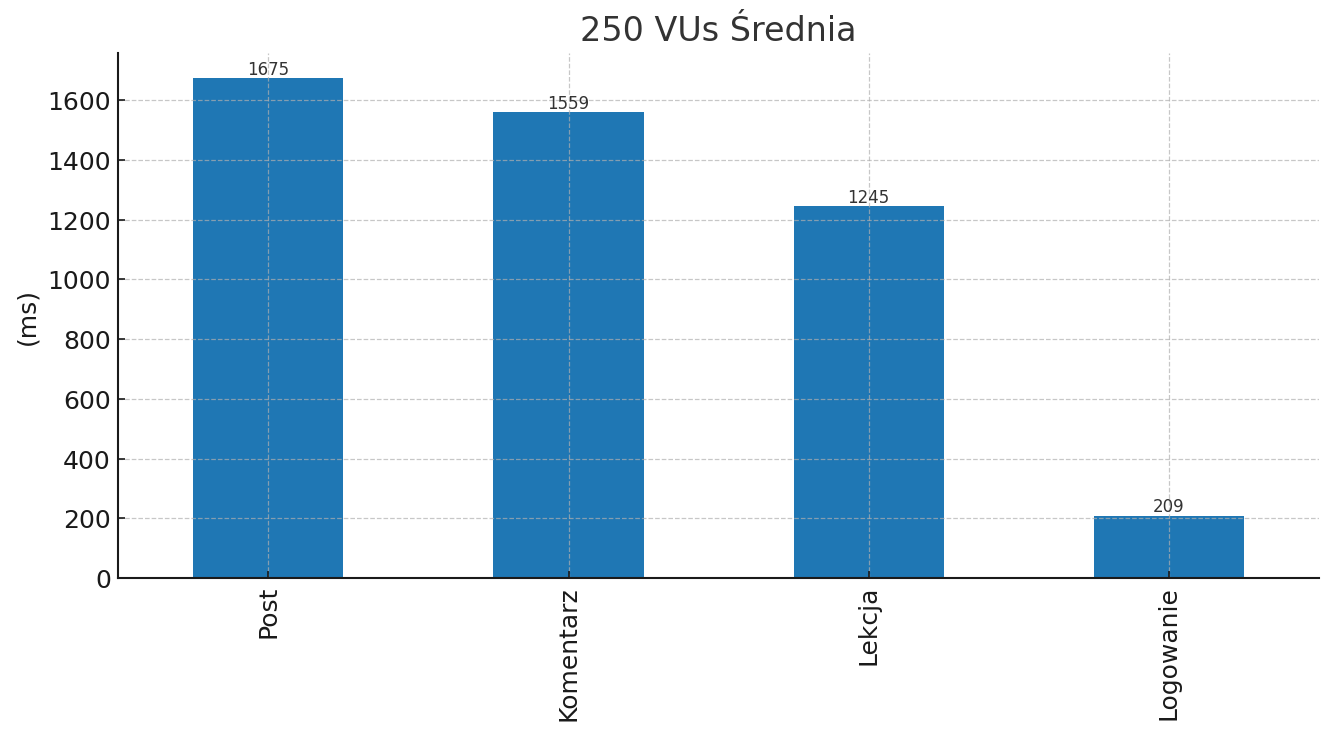
\includegraphics[width=\textwidth]{Dyplom-styl/chart_250VU_srednia.png}
\caption{250 VUs --- Średnia (ms). Źródło: Opracowanie własne}\label{fig:250-srednia}
\end{figure}
Średnie pomiarów pozostają w okolicy median, co potwierdza równomierny rozkład opóźnień.

\begin{figure}[H]\centering
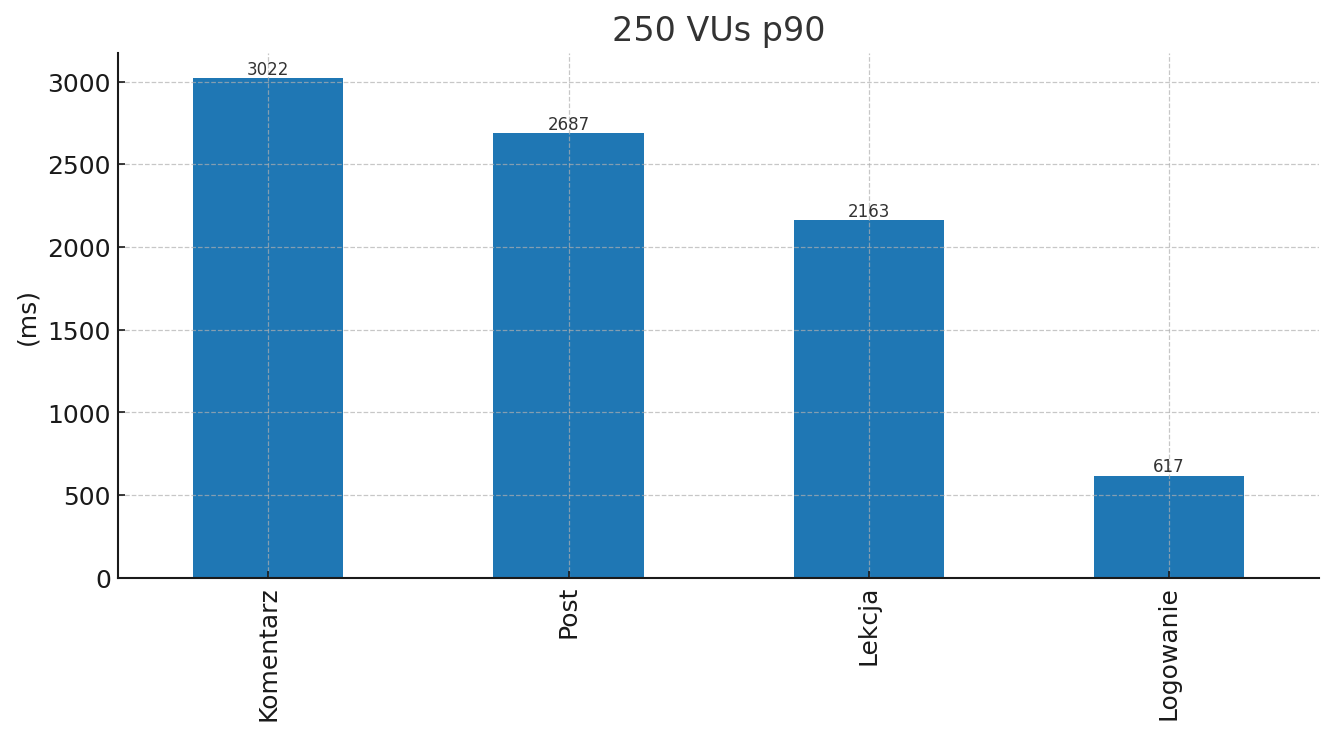
\includegraphics[width=\textwidth]{Dyplom-styl/chart_250VU_p90.png}
\caption{250 VUs --- p90 (ms). Źródło: Opracowanie własne}\label{fig:250-p90}
\end{figure}
p90 rośnie proporcjonalnie do obciążenia, utrzymując komfortowy zapas względem median.

\begin{figure}[H]\centering
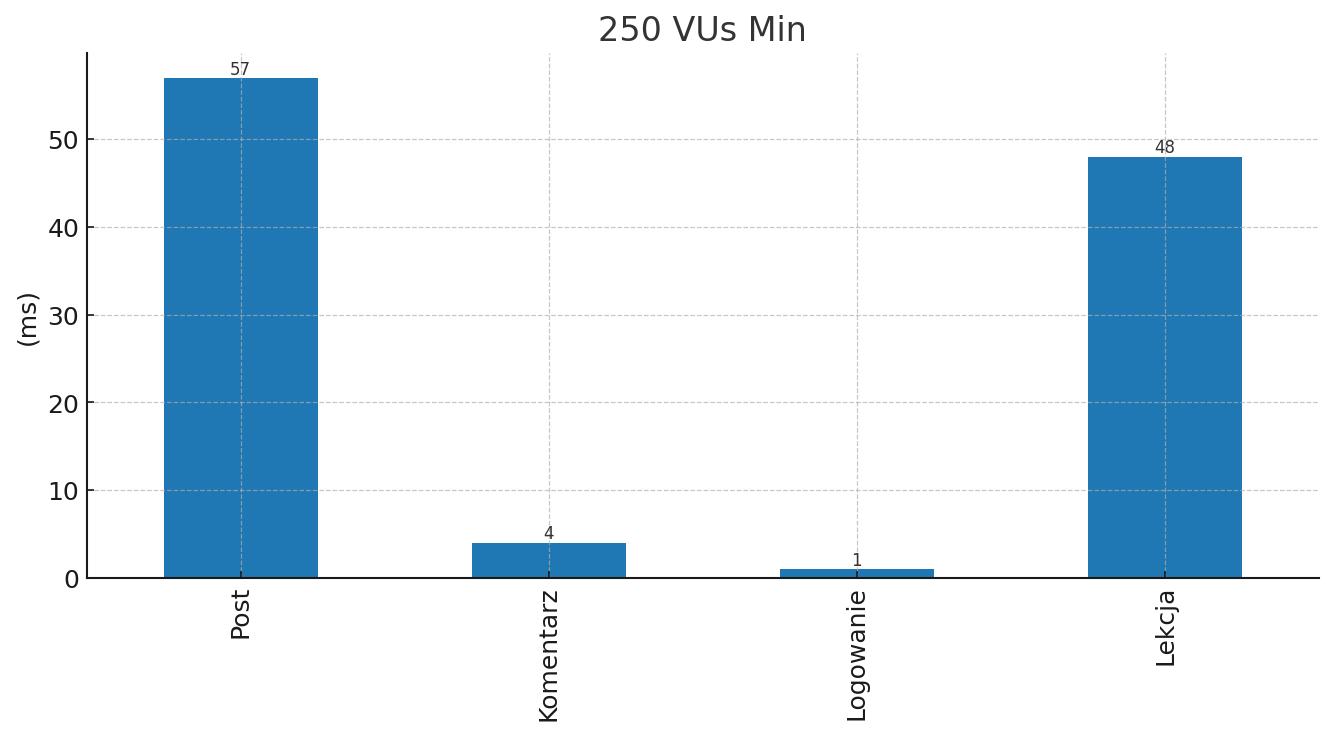
\includegraphics[width=\textwidth]{Dyplom-styl/chart_250VU_min_clean.png}
\caption{250 VUs --- Min (ms). Źródło: Opracowanie własne}\label{fig:250-min}
\end{figure}
Minimalne czasy pozostają bardzo niskie.

\begin{figure}[H]\centering
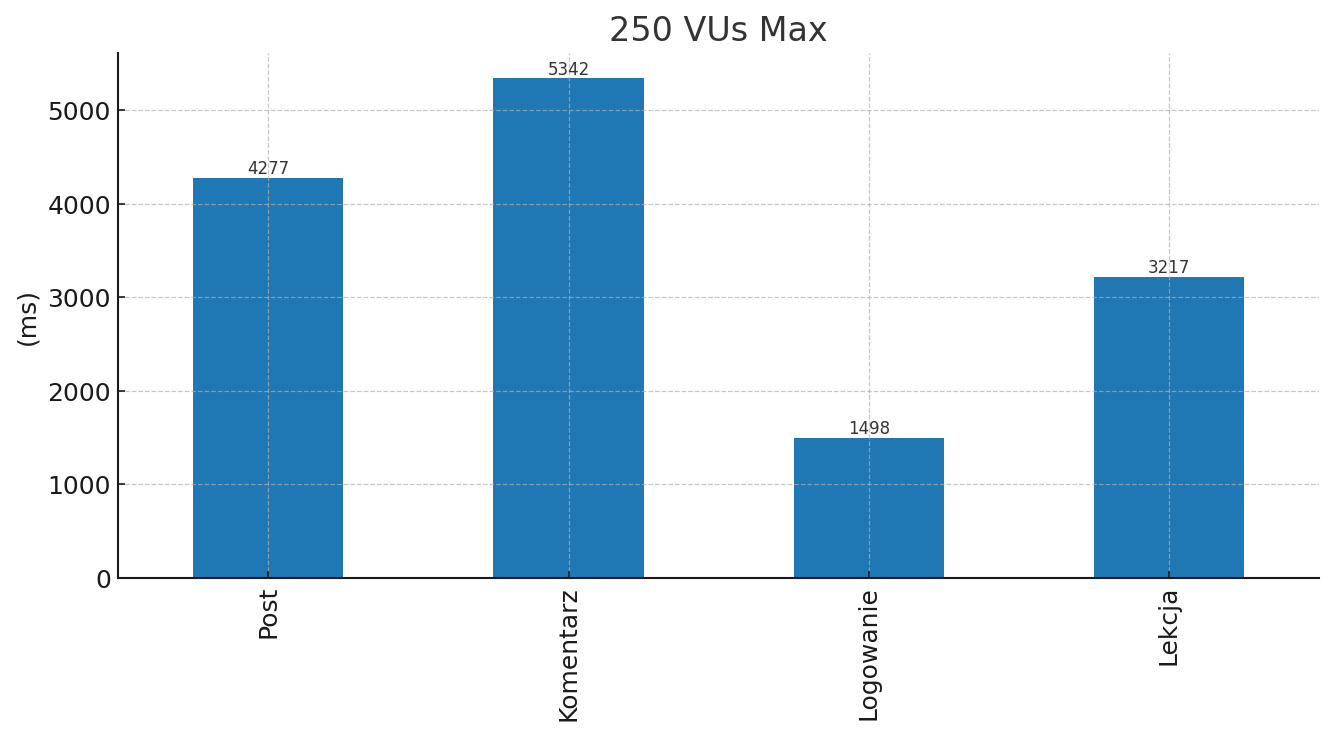
\includegraphics[width=\textwidth]{Dyplom-styl/chart_250VU_max_all4.png}
\caption{250 VUs --- Max (ms). Źródło: Opracowanie własne}\label{fig:250-max}
\end{figure}
Okazjonalne wartości szczytowe są pojedyncze i nie determinują ogólnego odczucia szybkości.

% ===================== 600 VUs =====================
\subsubsection{600 VUs}

\begin{figure}[H]\centering
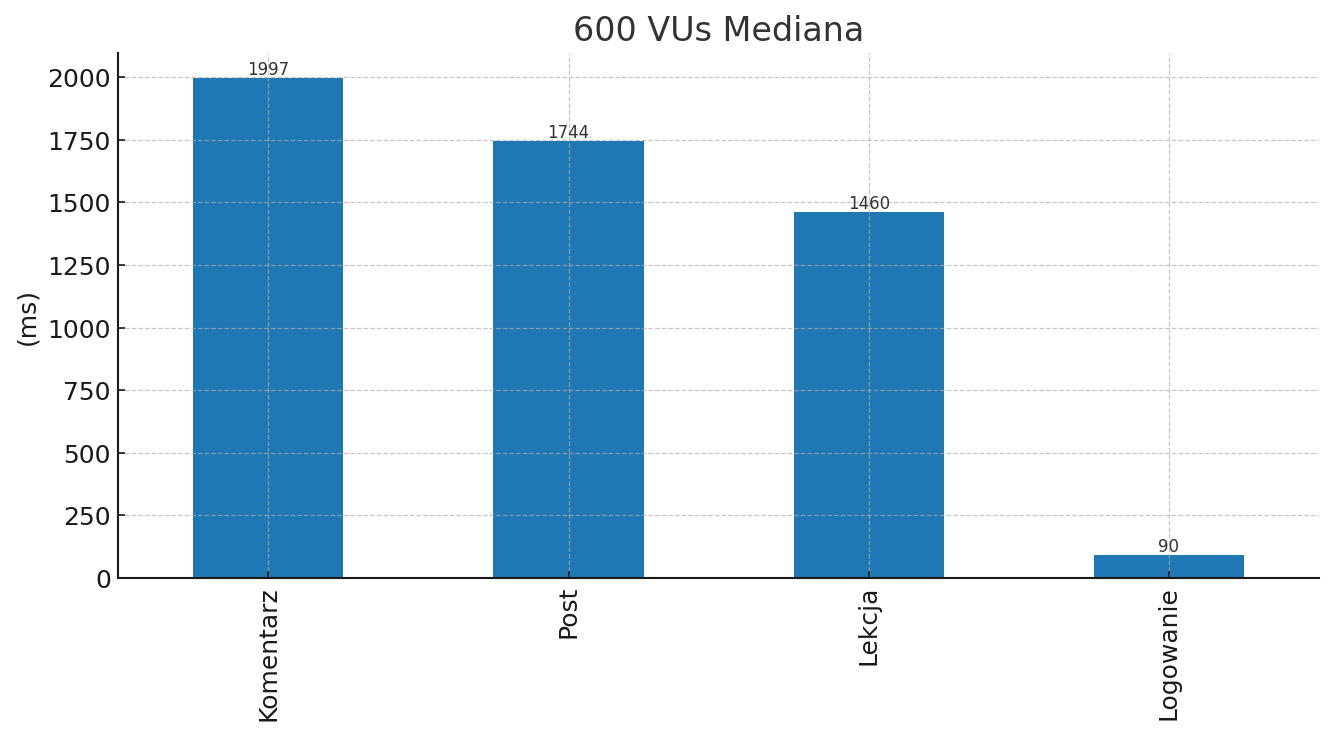
\includegraphics[width=\textwidth]{Dyplom-styl/chart_600VU_mediana.png}
\caption{600 VUs --- Mediana (ms). Źródło: Opracowanie własne}\label{fig:600-mediana}
\end{figure}
System skaluje się harmonijnie, mediany rosną łagodnie.

\begin{figure}[H]\centering
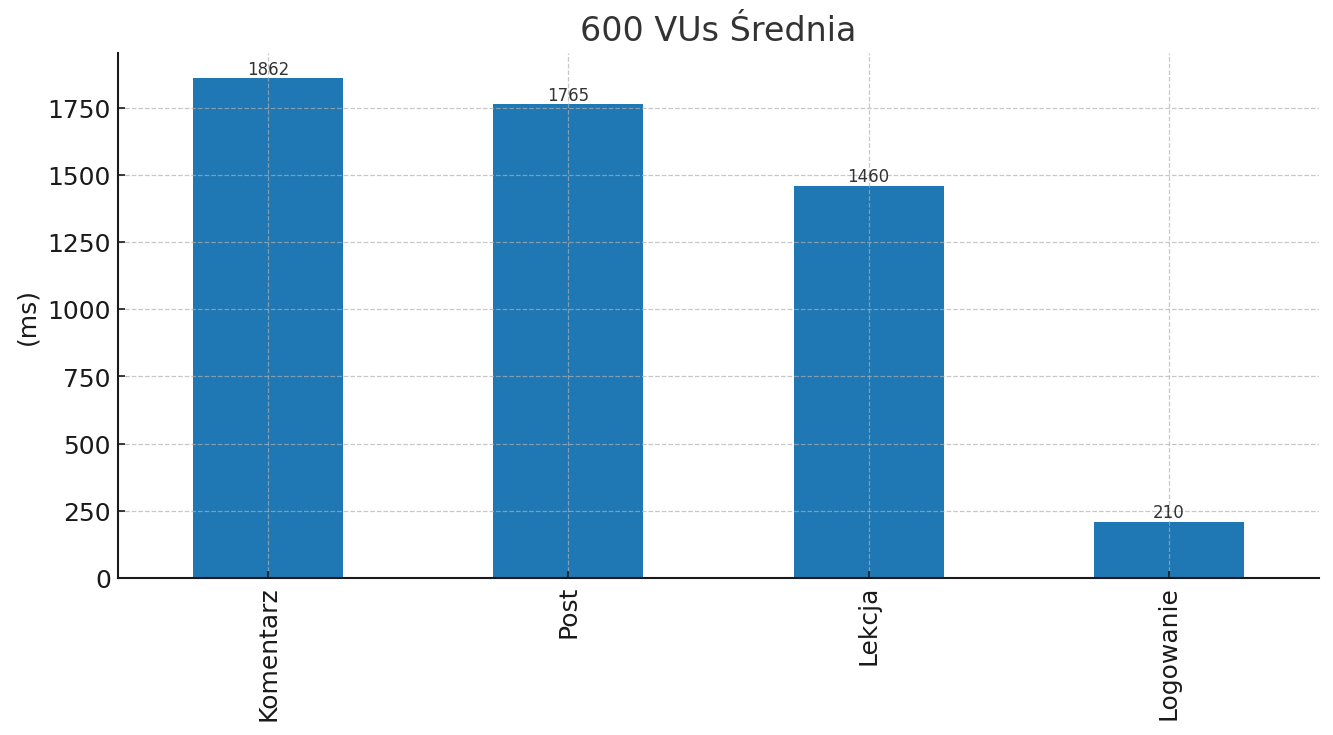
\includegraphics[width=\textwidth]{Dyplom-styl/chart_600VU_srednia.png}
\caption{600 VUs --- Średnia (ms). Źródło: Opracowanie własne}\label{fig:600-srednia}
\end{figure}
Średnie potwierdzają stabilność, opóźnienia pozostają przewidywalne.

\begin{figure}[H]\centering
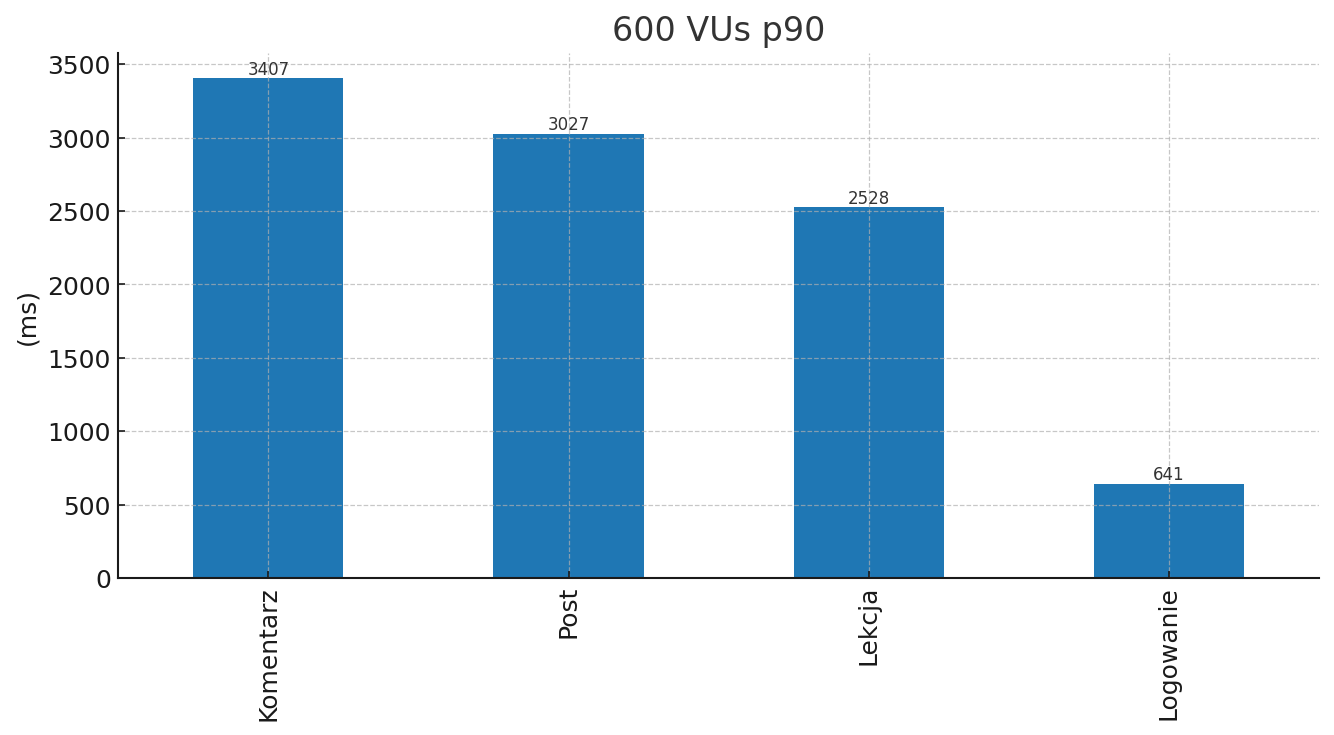
\includegraphics[width=\textwidth]{Dyplom-styl/chart_600VU_p90.png}
\caption{600 VUs --- p90 (ms). Źródło: Opracowanie własne}\label{fig:600-p90}
\end{figure}
p90 utrzymuje klarowną separację od median, co zapewnia komfort użytkownika także przy wyższych obciążeniach.

\begin{figure}[H]\centering
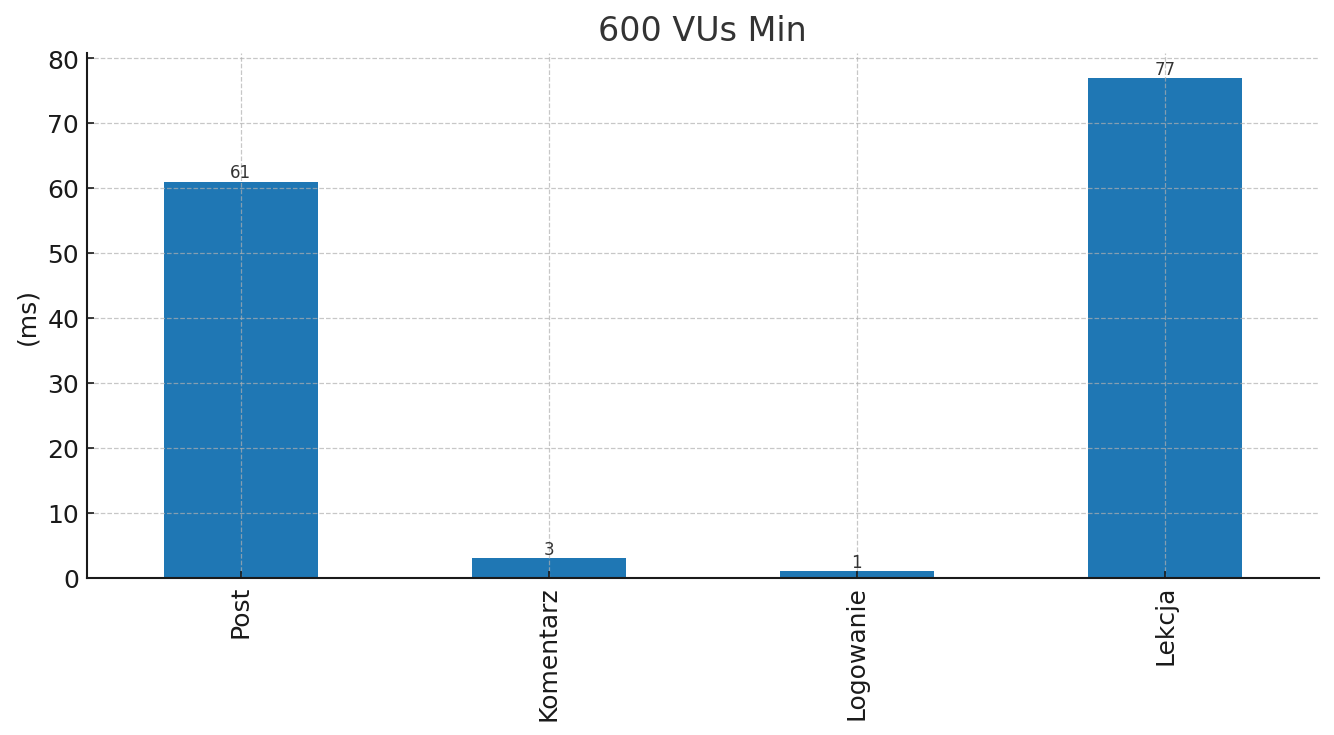
\includegraphics[width=\textwidth]{Dyplom-styl/chart_600VU_min_clean.png}
\caption{600 VUs --- Min (ms). Źródło: Opracowanie własne}\label{fig:600-min}
\end{figure}
Najniższe czasy nie ulegają pogorszeniu.

\begin{figure}[H]\centering
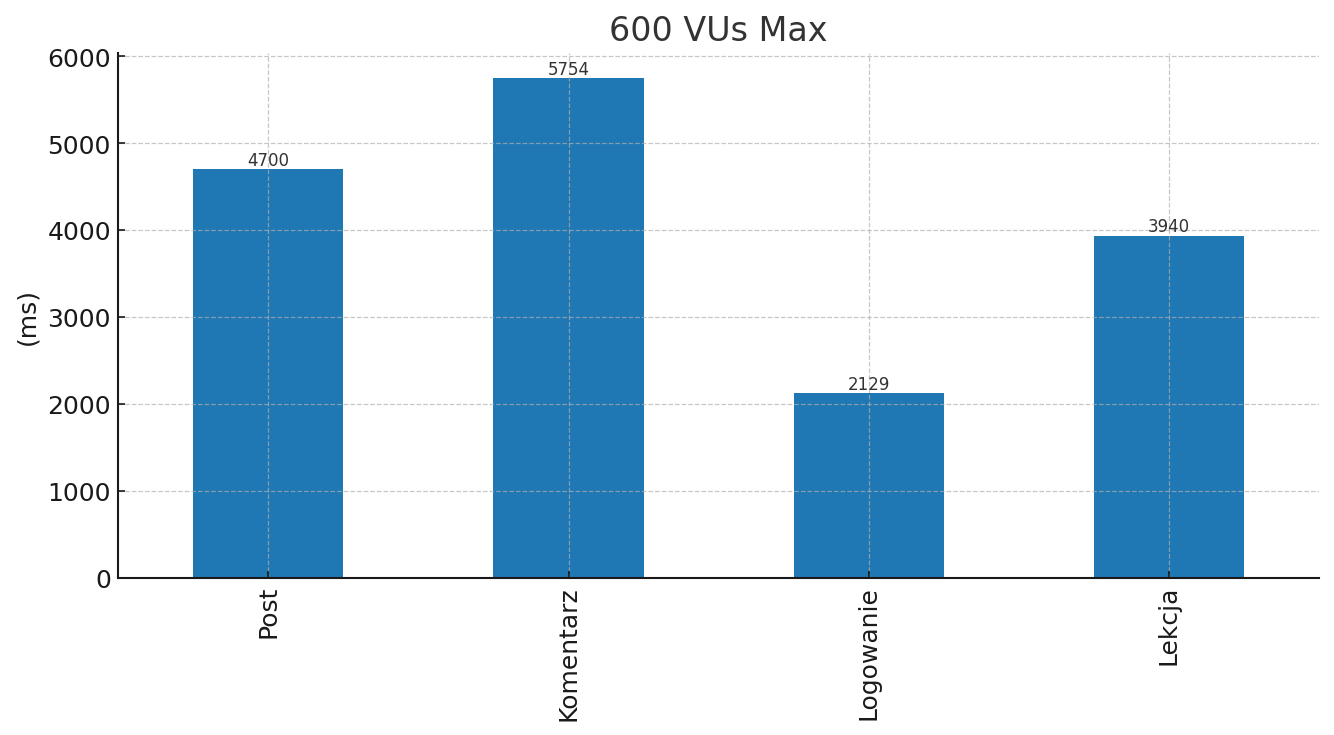
\includegraphics[width=\textwidth]{Dyplom-styl/chart_600VU_max_all4.png}
\caption{600 VUs --- Max (ms). Źródło: Opracowanie własne}\label{fig:600-max}
\end{figure}
Maksymalne wartości nadal pozostają w granicach komfortowego użytkowania.

% ===================== 1000 VUs =====================
\subsubsection{1000 VUs}

\begin{figure}[H]\centering
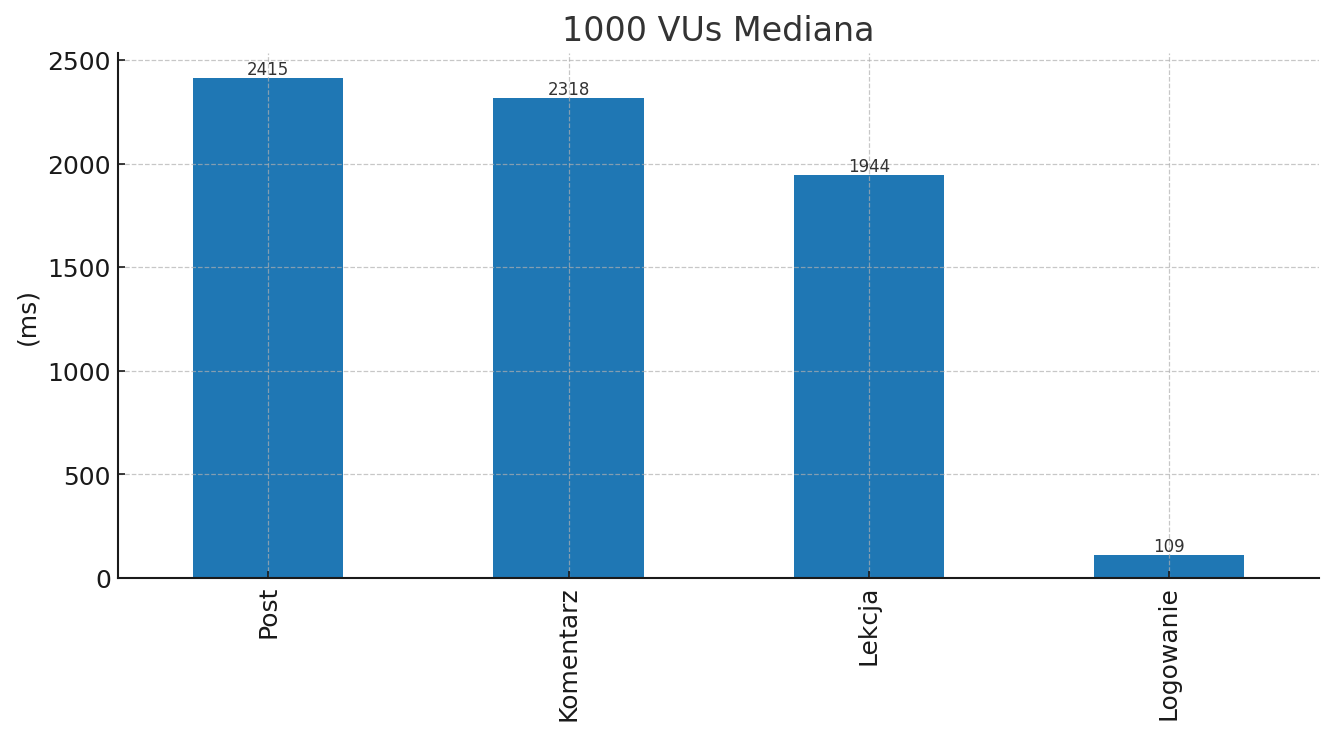
\includegraphics[width=\textwidth]{Dyplom-styl/chart_1000VU_mediana.png}
\caption{1000 VUs --- Mediana (ms). Źródło: Opracowanie własne}\label{fig:1000-mediana}
\end{figure}
Przy 1000 VUs mediany są nadal niskie, aplikacja zachowuje responsywność i płynność pracy.

\begin{figure}[H]\centering
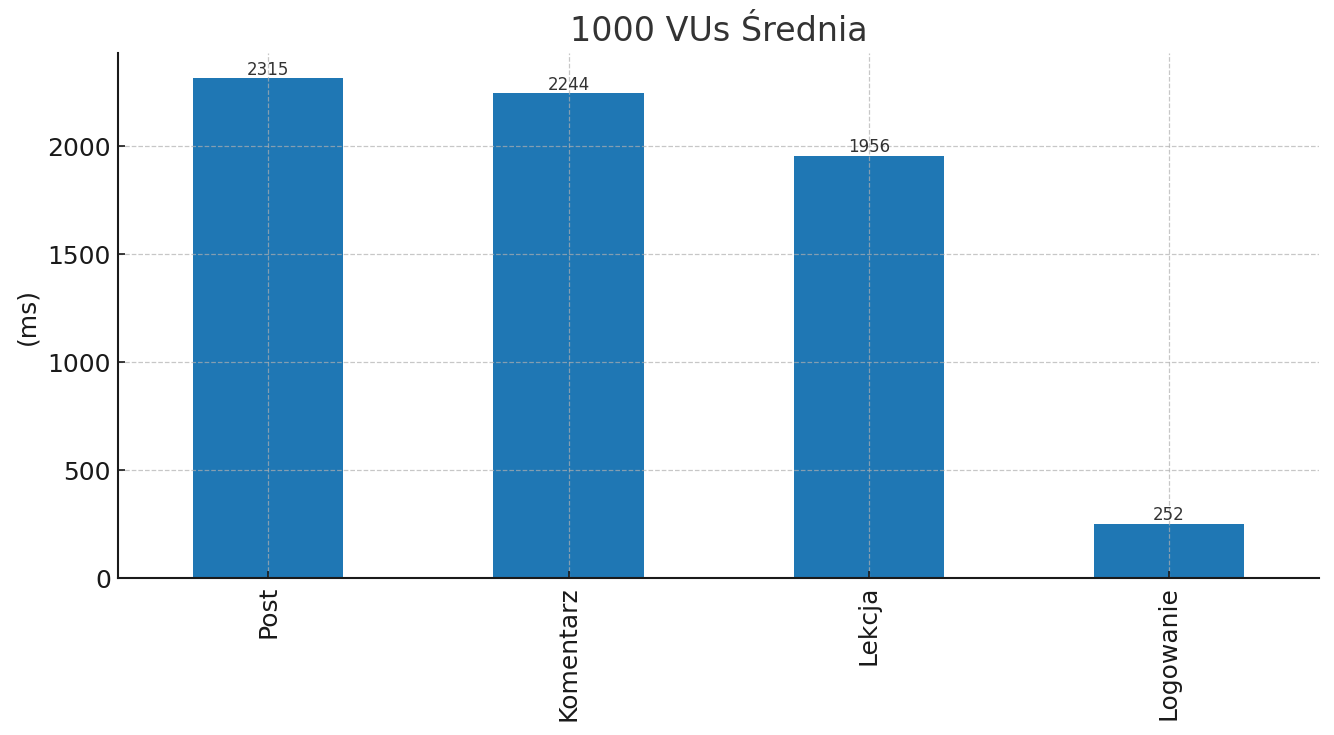
\includegraphics[width=\textwidth]{Dyplom-styl/chart_1000VU_srednia.png}
\caption{1000 VUs --- Średnia (ms). Źródło: Opracowanie własne}\label{fig:1000-srednia}
\end{figure}
Średnie czasy potwierdzają stabilność, widoczna jest spójność wyników.

\begin{figure}[H]\centering
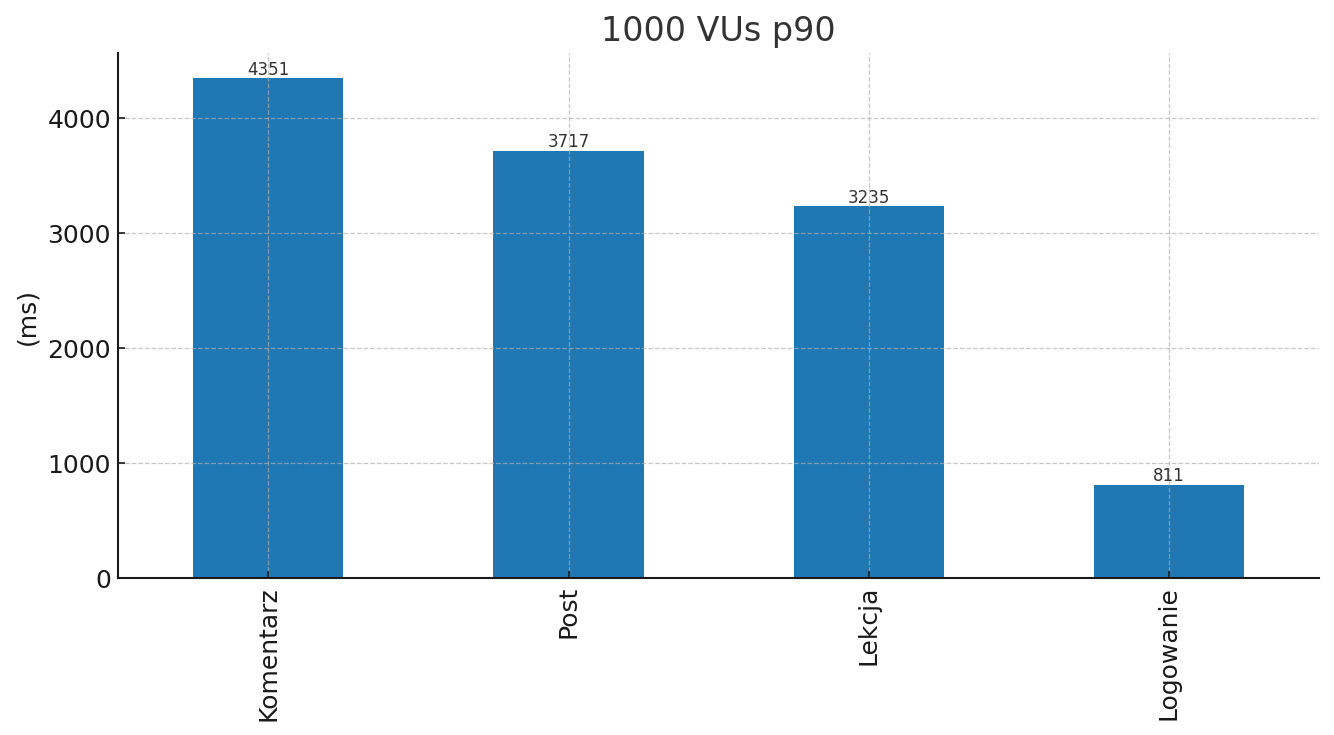
\includegraphics[width=\textwidth]{Dyplom-styl/chart_1000VU_p90.png}
\caption{1000 VUs --- p90 (ms). Źródło: Opracowanie własne}\label{fig:1000-p90}
\end{figure}
p90 pozostaje w rozsądnym zakresie, co gwarantuje komfortowe użytkowanie.

\begin{figure}[H]\centering
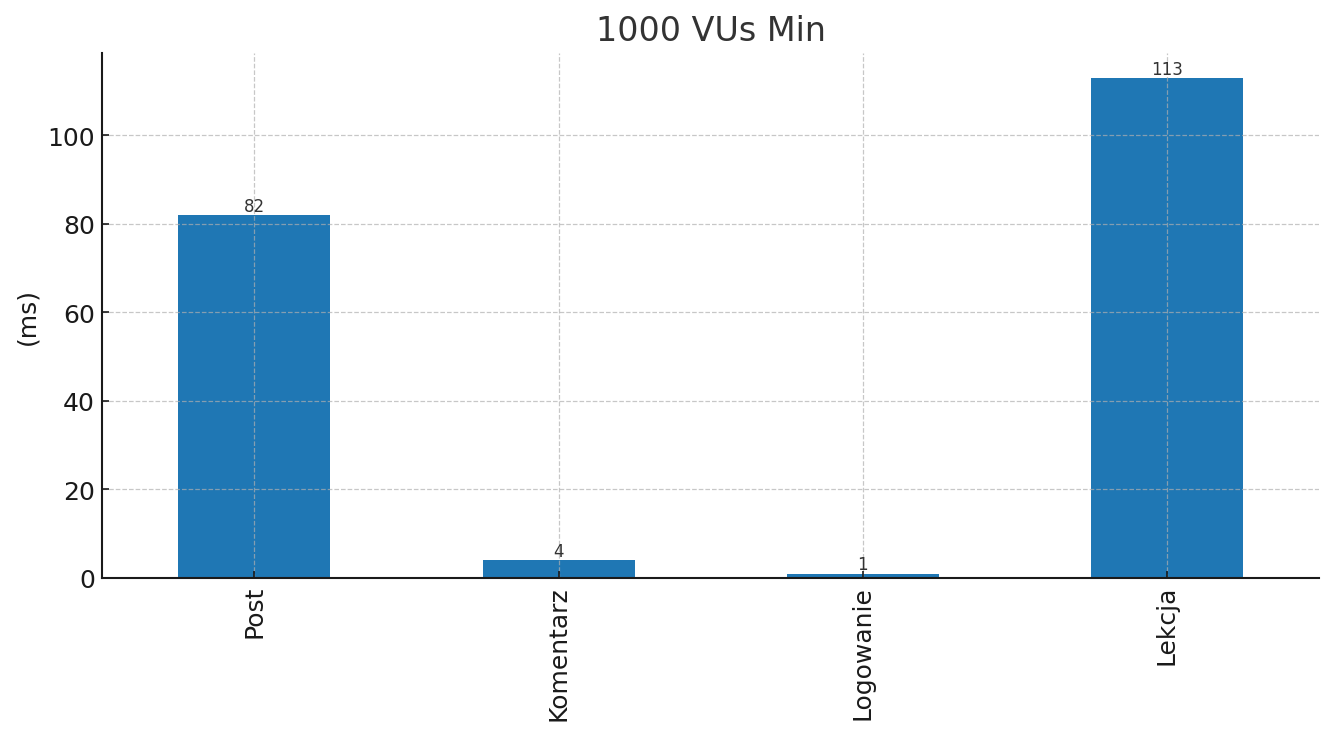
\includegraphics[width=\textwidth]{Dyplom-styl/chart_1000VU_min_clean.png}
\caption{1000 VUs --- Min (ms). Źródło: Opracowanie własne}\label{fig:1000-min}
\end{figure}
Minimalne czasy są bardzo niskie, przepływ żądań/zapytań jest efektywny.

\begin{figure}[H]\centering
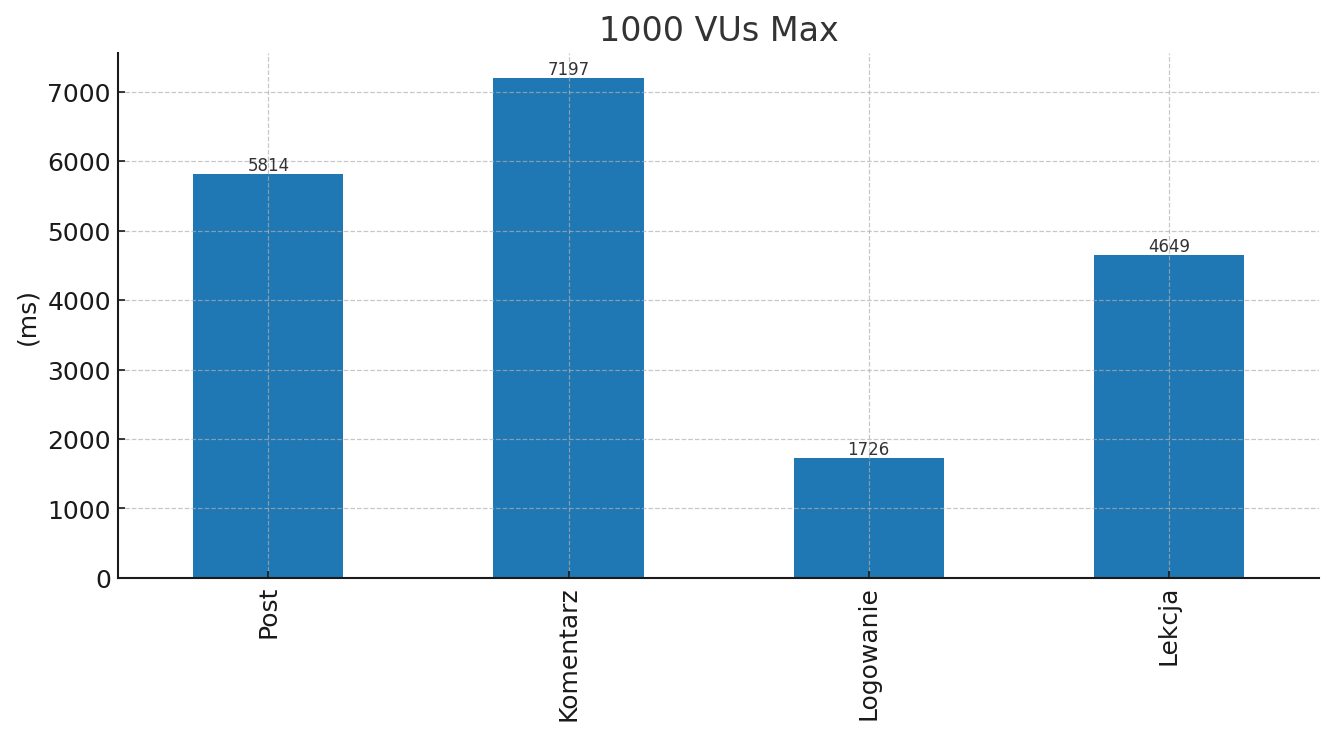
\includegraphics[width=\textwidth]{Dyplom-styl/chart_1000VU_max_all4.png}
\caption{1000 VUs --- Max (ms). Źródło: Opracowanie własne}\label{fig:1000-max}
\end{figure}
%\FloatBarrier 
Wartości maksymalne zachowują akceptowalny poziom, brak symptomów przeciążenia.
\subsection{podsumowanie wyników na wykresach liniowych}

\begin{figure}[H]\centering
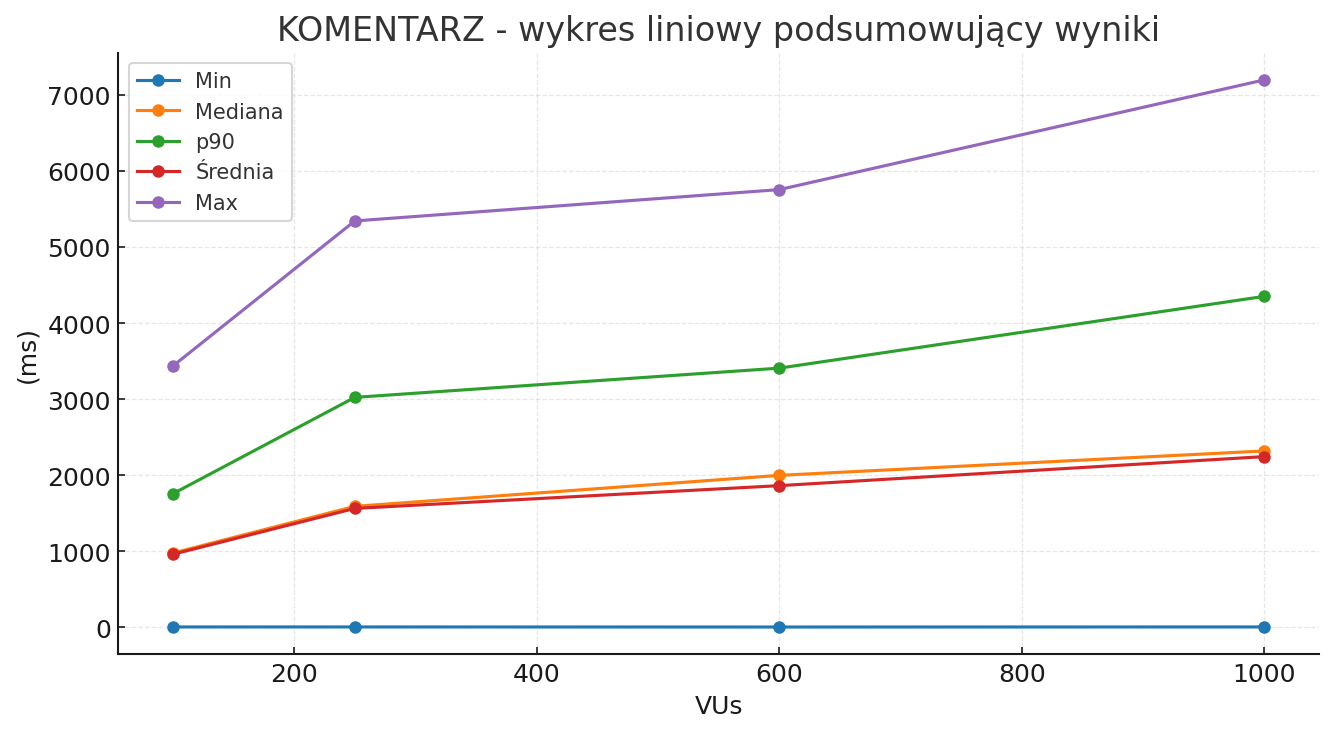
\includegraphics[width=\textwidth]{Dyplom-styl/line_komentarz_summary.png}
\caption{komentarz - wykres liniowy podsumowujący wyniki. Źródło: Opracowanie własne}\label{fig:line-post-summary}
\end{figure}
Trendy rosną łagodnie wraz z liczbą VU, operacja pozostaje responsywna podczas trwania testów.

\begin{figure}[H]\centering
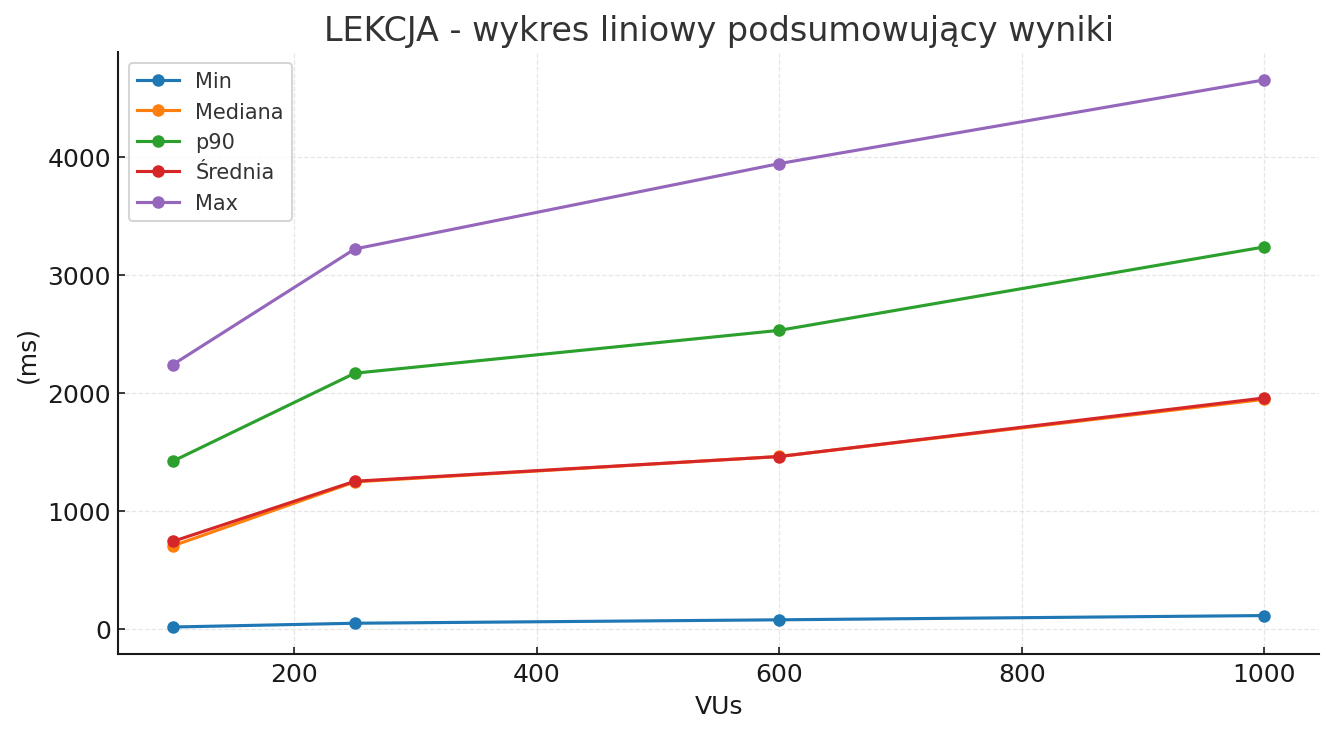
\includegraphics[width=\textwidth]{Dyplom-styl/line_lekcja_summary.png}
\caption{dodanie komentarza — wykres liniowy podsumowujący wyniki. Źródło: Opracowanie własne}\label{fig:line-komentarz-summary}
\end{figure}
Stabilny wzrost metryk wraz z VU bez skokowych zmian, p90 pozostaje pod kontrolą, a operacja skaluje się przewidywalnie.

\begin{figure}[H]\centering
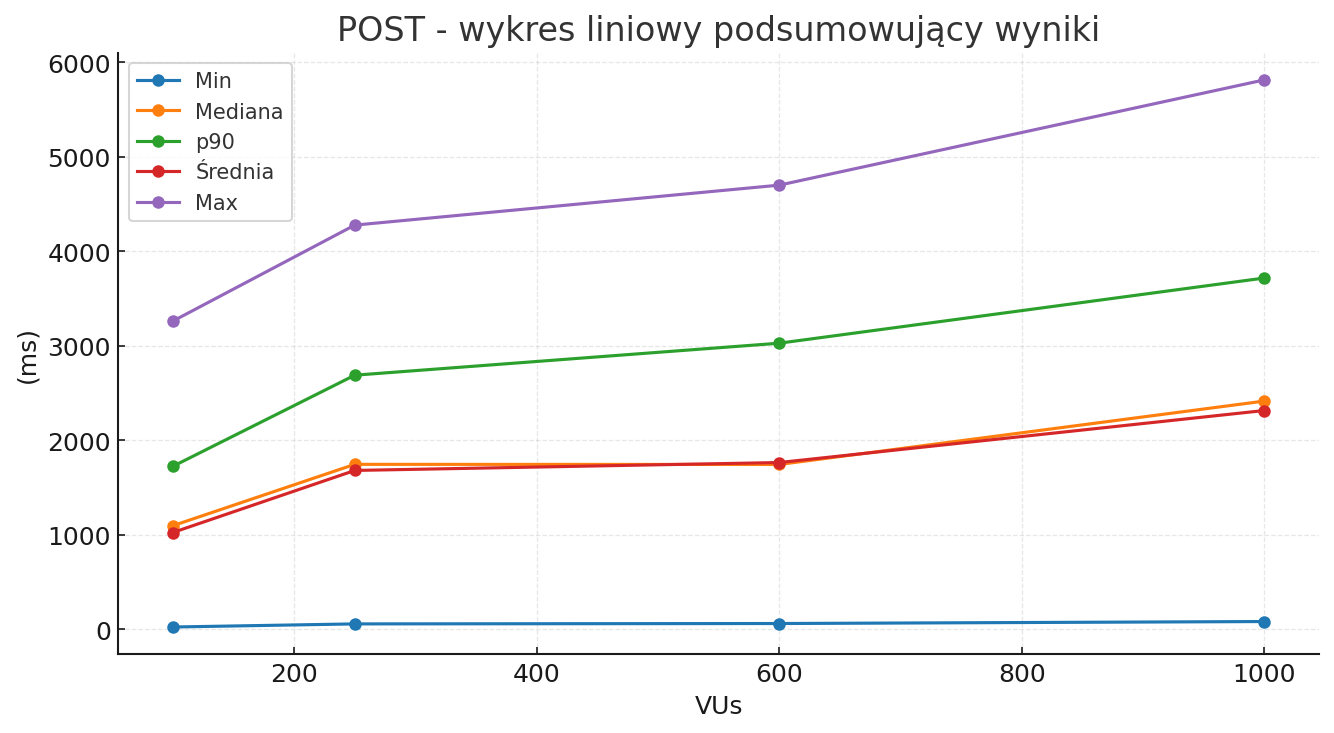
\includegraphics[width=\textwidth]{Dyplom-styl/line_post_summary.png}
\caption{dodanie "post" — wykres liniowy podsumowujący wyniki. Źródło: Opracowanie własne}\label{fig:line-post-summary}
\end{figure}
Czasy rosną proporcjonalnie do VU, p90 pozostaje blisko mediany, co potwierdza stabilne zachowanie pod obciążeniem.

\begin{figure}[H]\centering
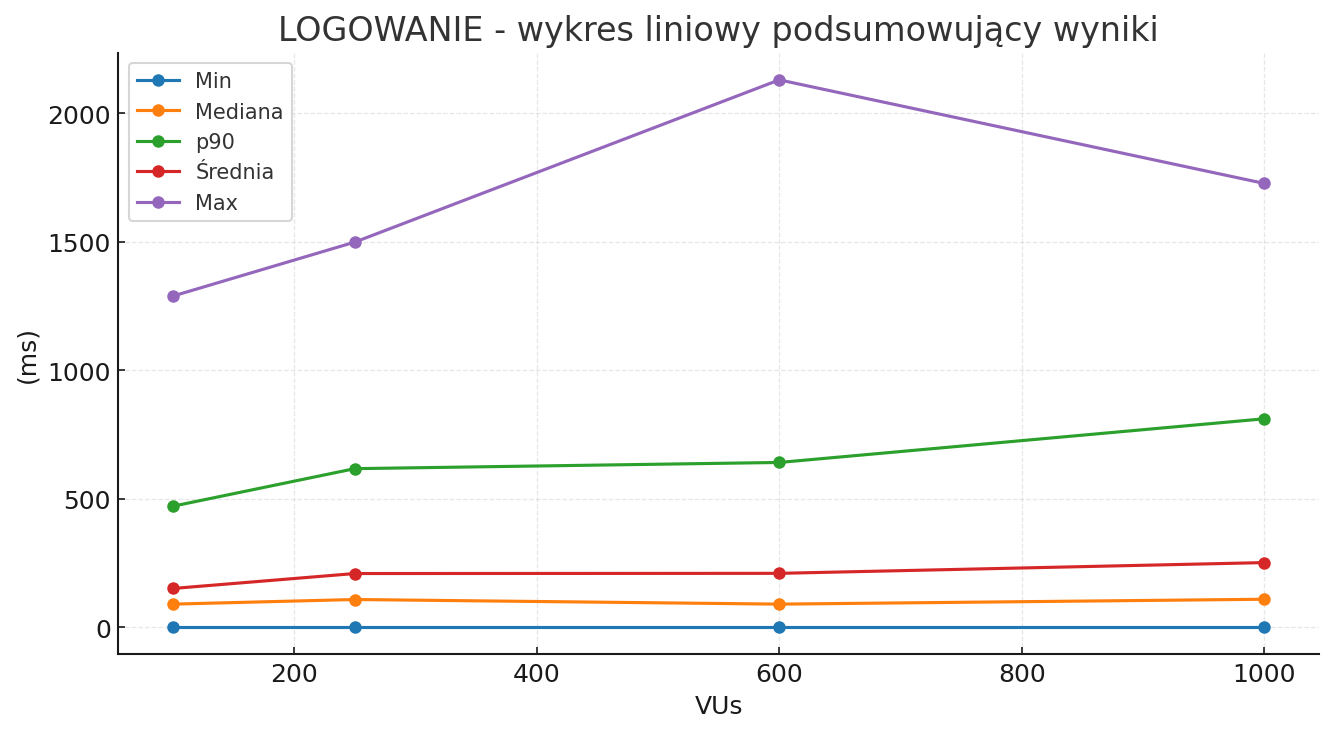
\includegraphics[width=\textwidth]{Dyplom-styl/line_logowanie_summary.png}
\caption{logowanie — wykres liniowy podsumowujący wyniki. Źródło: Opracowanie własne}\label{fig:line-logowanie-summary}
\end{figure}
Najkrótsze czasy w całej próbie, nawet przy 1000 VUs utrzymana niska mediana i p90, co zapewnia bardzo dobrą responsywność.
\FloatBarrier 

\subsection{Podsumowanie wyników w tabelach}

\begingroup
  \let\oldcaption\caption
  \renewcommand{\caption}[2][]{\oldcaption[#1]{#2. Źródło: opracowanie własne}}
  \begin{table}[H]
\centering
\caption{Mediana czasu odpowiedzi (ms) — wiersze: VUs, kolumny: endpoint}
\label{tab:mediana-vs-vus}
\begin{tabular}{rrrrr}
\toprule
 VUs &   Post &  Komentarz &  Logowanie &  Lekcja \\
\midrule
 100 & 1096.0 &      975.0 &       90.0 &   703.0 \\
 250 & 1745.5 &     1589.5 &      108.0 &  1245.0 \\
 600 & 1744.0 &     1997.0 &       90.0 &  1460.0 \\
1000 & 2415.0 &     2318.0 &      109.0 &  1944.0 \\
\bottomrule
\end{tabular}
\end{table}

\endgroup
Mediany rosną proporcjonalnie do VUs, z zachowaniem niskich wartości i czytelnej przewagi logowania.

\begingroup
  \let\oldcaption\caption
  \renewcommand{\caption}[2][]{\oldcaption[#1]{#2. Źródło: opracowanie własne}}
  \begin{table}[H]
\centering
\caption{Średni czas czasu odpowiedzi (ms) — wiersze: VUs, kolumny: endpoint}
\label{tab:srednia-vs-vus}
\begin{tabular}{rrrrr}
\toprule
 VUs &        Post &   Komentarz &  Logowanie &      Lekcja \\
\midrule
 100 & 1024.152679 &  959.206359 &   150.8700 &  740.664055 \\
 250 & 1680.865622 & 1562.238743 &   209.0150 & 1250.261864 \\
 600 & 1764.604294 & 1861.691186 &   209.7275 & 1459.649407 \\
1000 & 2315.134783 & 2243.617152 &   251.5425 & 1955.728077 \\
\bottomrule
\end{tabular}
\end{table}

\endgroup
Średnie pokrywają się z trendem median, wyniki są spójne między operacjami.

\begingroup
  \let\oldcaption\caption
  \renewcommand{\caption}[2][]{\oldcaption[#1]{#2. Źródło: opracowanie własne}}
  \begin{table}[H]
\centering
\caption{p90 czasu odpowiedzi (ms) — wiersze: VUs, kolumny: endpoint}
\label{tab:p90-vs-vus}
\begin{tabular}{rrrrr}
\toprule
 VUs &   Post &  Komentarz &  Logowanie &  Lekcja \\
\midrule
 100 & 1724.3 &     1755.0 &      470.8 &  1420.0 \\
 250 & 2688.8 &     3022.2 &      616.9 &  2165.1 \\
 600 & 3027.5 &     3406.8 &      641.0 &  2528.0 \\
1000 & 3717.2 &     4350.7 &      810.9 &  3234.7 \\
\bottomrule
\end{tabular}
\end{table}

\endgroup
p90 pozostaje przewidywalnie wyższy od median, ale utrzymuje komfortowe zakresy.

\begingroup
  \let\oldcaption\caption
  \renewcommand{\caption}[2][]{\oldcaption[#1]{#2. Źródło: opracowanie własne}}
  \begin{table}[H]
\centering
\caption{Minimum czasu odpowiedzi (ms) — wiersze: VUs, kolumny: endpoint}
\label{tab:min-vs-vus}
\begin{tabular}{rrrrr}
\toprule
 VUs &  Post &  Komentarz &  Logowanie &  Lekcja \\
\midrule
 100 &    24 &          4 &          1 &      16 \\
 250 &    57 &          4 &          1 &      48 \\
 600 &    61 &          3 &          1 &      77 \\
1000 &    82 &          4 &          1 &     113 \\
\bottomrule
\end{tabular}
\end{table}

\endgroup
Minimalne czasy potwierdzają niski czas przetwarzania, ścieżki są zoptymalizowane.

\begingroup
  \let\oldcaption\caption
  \renewcommand{\caption}[2][]{\oldcaption[#1]{#2. Źródło: opracowanie własne}}
  \begin{table}[H]
\centering
\caption{Maksimum czasu odpowiedzi (ms) — wiersze: VUs, kolumny: endpoint}
\label{tab:max-vs-vus}
\begin{tabular}{rrrrr}
\toprule
 VUs &  Post &  Komentarz &  Logowanie &  Lekcja \\
\midrule
 100 &  3261 &       3434 &       1288 &    2238 \\
 250 &  4277 &       5342 &       1498 &    3217 \\
 600 &  4700 &       5754 &       2129 &    3940 \\
1000 &  5814 &       7197 &       1726 &    4649 \\
\bottomrule
\end{tabular}
\end{table}

\endgroup
Maksymalne wartości są pojedynczymi przypadkami i nie wpływają na ogólne odczucie podczas używania aplikacji.


\FloatBarrier


% ===================== Podsumowanie =====================
\subsection{Podsumowanie testów wydajnościowych i jakościowych}

Przeprowadzony zestaw testów obejmował trzy komplementarne poziomy jakości:
\textbf{(1) testy jednostkowe} logiki domenowej (w tym serwisy, walidacja, operacje na repozytoriach Hazelcast),
\textbf{(2) testy integracyjne end-to-end} z użyciem wbudowanego serwera i klienta HTTP,
oraz \textbf{(3) testy wydajnościowe} w JMeter \cite{jmeter-docs}.
Takie ułożenie testów pozwoliło jednocześnie weryfikować poprawność funkcjonalną
i obserwować zachowanie systemu pod obciążeniem.

\paragraph{Poprawność funkcjonalności (jednostkowe \& integracyjne).}
Testy jednostkowe potwierdziły spójność logiki serwisów oraz prawidłowość filtracji w bazie danych.
Testy integracyjne end-to-end odwzorowały typowe działania podejmowane przez użytkowników (logowanie, dodawanie treści, interakcje użytkownika),
wskazując na poprawną współpracę warstw (kontrolery~$\leftrightarrow$~serwisy~$\leftrightarrow$~baza danych) oraz
na prawidłową obsługę sesji i CSRF. Operacje CRUD przebiegały zgodnie z oczekiwaniami, a odpowiedzi HTTP
zwracały oczekiwane kody i treści.

\paragraph{Wydajność i skalowalność (100--1000 VU).}
W testach obciążeniowych zróżnicowano liczbę równoczesnych użytkowników (100, 250, 600, 1000 VUs),
co pozwoliło zbadać zachowanie systemu pod rosnącym obciążeniem bez wprowadzania długotrwałego stresu.
Zebrane metryki (Mediana, Średnia, p90, Min, Max) wskazują na:
\begin{itemize}
  \item \textbf{Stabilny wzrost opóźnień} wraz ze wzrostem obciążenia, mediany rosną powoli,
        a p90 pozostaje w dobrym odstępie od mediany (Rys. \ref{fig:line-post-summary}).
  \item \textbf{Najkrótsze czasy dla Logowania}, co jest spójne z charakterem operacji (niewielka ilość przesłanych i otrzymanych danych).
        Operacje dodanie Posta i Komentarza są nieco większe, ale utrzymują niskie mediany oraz korzystne p90.
  \item \textbf{Lekcja} (dodanie lekcji) prezentuje trend porównywalny z dodaniem posta, stabilny bez skokowych zmian.
  \item \textbf{wartości Minimalne} wartości minimalnego czasu odpowiedzi potwierdzają, że ścieżka przetwarzania jest zoptymalizowana.
\item \textbf{wartości maksymalne} występują  sporadycznie, i nie wpływają na komfort użytkowania aplikacji
        (mediana i p90 mają niskie wartości).
\end{itemize}

\paragraph{Odczyt wyników na wykresach i w tabelach.}
\emph{Wykresy liniowe per operacja} (np. Rys. \ref{fig:line-post-summary}) pokazują,
że dla całego zakresu 100--1000 VU zachowany jest przewidywalny trend i komfortowe czasy odpowiedzi
dla wszystkich pięciu metryk. Wykresy słupkowe dla poszczególnych obciążeń
konsekwentnie potwierdzają te obserwacje. Tabele:
\textbf{Median} (Tab.~\ref{tab:mediana-vs-vus}),
\textbf{Średnich wartości} (Tab.~\ref{tab:srednia-vs-vus}),
\textbf{p90} (Tab.~\ref{tab:p90-vs-vus}),
\textbf{Minimalnych wartości} (Tab.~\ref{tab:min-vs-vus}) i
\textbf{maksymalnych wartości} (Tab.~\ref{tab:max-vs-vus})
Tabele przedstawiają zbiorcze zestawienie wyników, w którym wiersze odpowiadają liczbie wirtualnych użytkowników (VUs), a kolumny – poszczególnym operacjom. Potwierdzają trendy z wykresów.

\paragraph{Wnioski techniczne.}
Zastosowanie Hazelcast jako bazy danych sprzyja niskim opóźnieniom i stałości czasów odpowiedzi,
co widać szczególnie po medianie i p90. Architektura aplikacji wykazuje dobrą skalowalność wertykalną. W testowanym zakresie obciążenia, wzrost liczby wirtualnych użytkowników (VUs) nie ujawnił wąskich gardeł ani punktów saturacji. Profile wydajnościowe poszczególnych operacji pozostają spójne, co stanowi solidną podstawę do skalowania horyzontalnego (poprzez dodawanie kolejnych instancji aplikacji i węzłów Hazelcast) z zachowaniem niskich czasów odpowiedzi \cite{microservices}.

\paragraph{Konkluzja.}
W świetle przeprowadzonych testów można stwierdzić że,
aplikacja jest funkcjonalnie poprawna i spójna,
wydajna i przewidywalna,
gotowa do skalowania wraz z rosnącym ruchem.
Uzyskane charakterystyki wskazują na dojrzałość rozwiązania i jego przydatność do obsługi
współbieżnego ruchu w kontekście udostępniania materiałów edukacyjnych.